% \documentclass[lineno,twocolumn,endfloat,biblatex]{biophys-new}
\documentclass{biophys-new}
\usepackage[utf8]{inputenc}
\usepackage{graphicx}
\usepackage[colorlinks,allcolors=cyan!70!black]{hyperref}

% uncomment if using biblatex
% \addbibresource{sample.bib}

\usepackage{lipsum}

\title{Understanding the Free Energy Landscape of Phase Separation in Lipid Bilayer using Weighted Ensemble Molecular Dynamics}
\runningtitle{All plots with long captions} %% For page header

\author[1]{Ashlin Poruthoor}
\author[1,*]{Alan Grossfield}
\runningauthor{Poruthoor and Grossfield} %% For page header

\affil[1]{University of Rochester Medical Center, Rochester, NY 14620}

\corrauthor[*]{alan\_grossfield@urmc.rochester.edu}

% \papertype{Letters}
\papertype{Article}
% \papertype{Computational Tools}


\begin{document}

\begin{frontmatter}
\begin{abstract}

Lorem ipsum dolor sit amet, consectetur adipiscing elit, sed do eiusmod tempor incididunt ut labore et dolore magna aliqua. Ut enim ad minim veniam, quis nostrud exercitation ullamco laboris nisi ut aliquip ex ea commodo consequat. Duis aute irure dolor in reprehenderit in voluptate velit esse cillum dolore eu fugiat nulla pariatur. Excepteur sint occaecat cupidatat non proident, sunt in culpa qui officia deserunt mollit anim id est laborum.

\end{abstract}

\begin{sigstatement}

Lorem ipsum dolor sit amet, consectetur adipiscing elit, sed do eiusmod tempor incididunt ut labore et dolore magna aliqua. Ut enim ad minim veniam, quis nostrud exercitation ullamco laboris nisi ut aliquip ex ea commodo consequat. Duis aute irure dolor in reprehenderit in voluptate velit esse cillum dolore eu fugiat nulla pariatur. Excepteur sint occaecat cupidatat non proident, sunt in culpa qui officia deserunt mollit anim id est laborum

\end{sigstatement}

\end{frontmatter}

\section*{Introduction}

This is a place holder article template for our future paper. For time being, I will be using this 
space to publish all the plots that are being generated as a part of the analysis.

\section*{Methods}

Lorem ipsum dolor sit amet, consectetur adipiscing elit, sed do eiusmod tempor incididunt ut labore et dolore magna aliqua. Ut enim ad minim veniam, quis nostrud exercitation ullamco laboris nisi ut aliquip ex ea commodo consequat. Duis aute irure dolor in reprehenderit in voluptate velit esse cillum dolore eu fugiat nulla pariatur. Excepteur sint occaecat cupidatat non proident, sunt in culpa qui officia deserunt mollit anim id est laborum.

\section*{Results}

Lorem ipsum dolor sit amet, consectetur adipiscing elit, sed do eiusmod tempor incididunt ut labore et dolore magna aliqua. Ut enim ad minim veniam, quis nostrud exercitation ullamco laboris nisi ut aliquip ex ea commodo consequat. Duis aute irure dolor in reprehenderit in voluptate velit esse cillum dolore eu fugiat nulla pariatur. Excepteur sint occaecat cupidatat non proident, sunt in culpa qui officia deserunt mollit anim id est laborum.

\subsection*{All Figures}

\begin{figure}[hbt!]
\centering
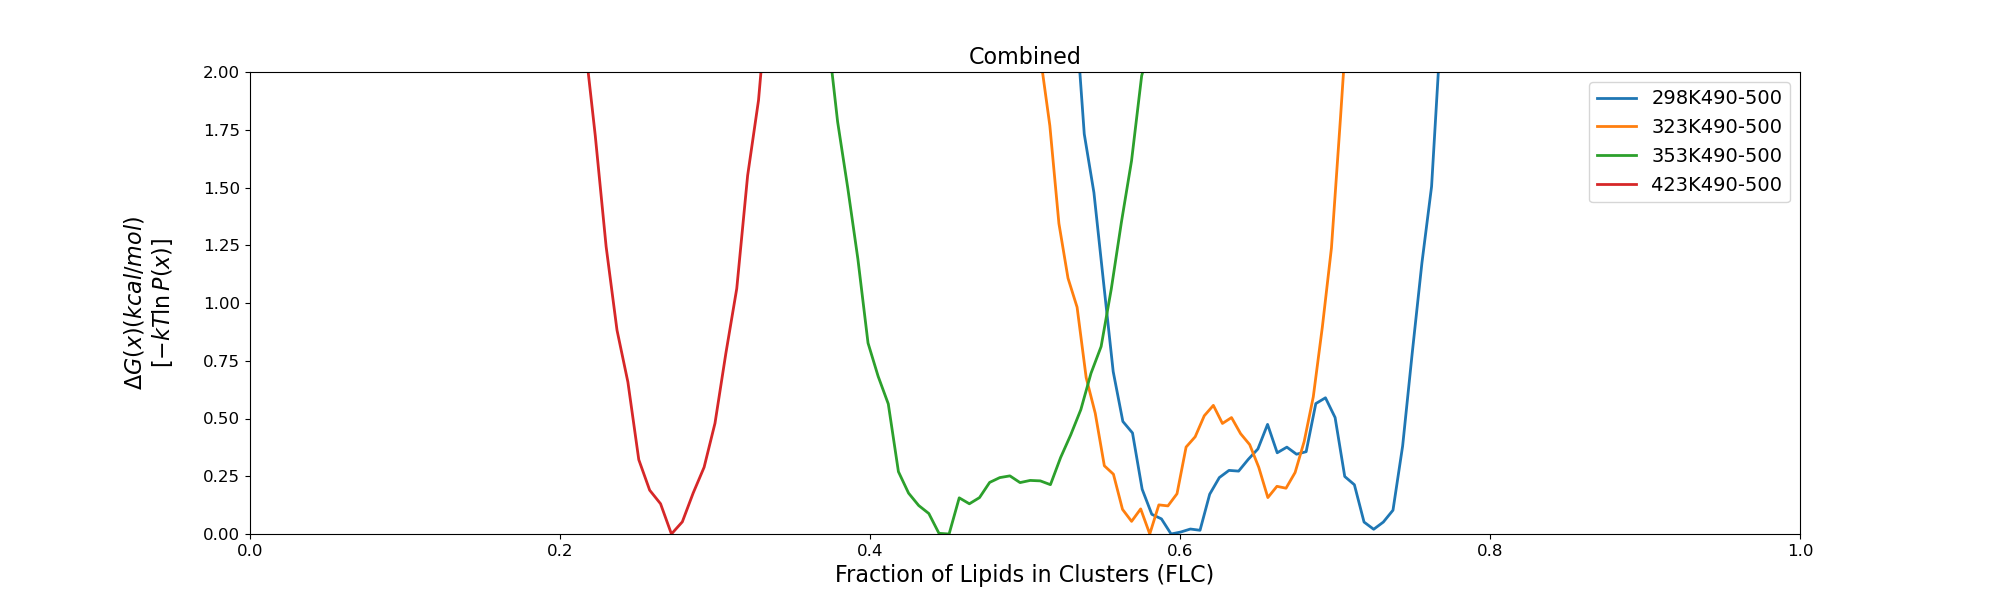
\includegraphics[width=1.1\linewidth]{all_plots/ClusterLipids2Total/DPPC_DIPC_CHOL/Average_DIPC_MULTI__ClusterLipids2Total.png}
\caption{Free Energy Landscape of \textbf{DIPC} system. Data from all four replicas has been combined using w\_multi\_west tool. All the FES are calculated by averaging over the iteration window 490 - 500. Note that 353K is an interesting outlier}
\label{fig:view}

\end{figure}

\begin{figure}[hbt!]
\centering
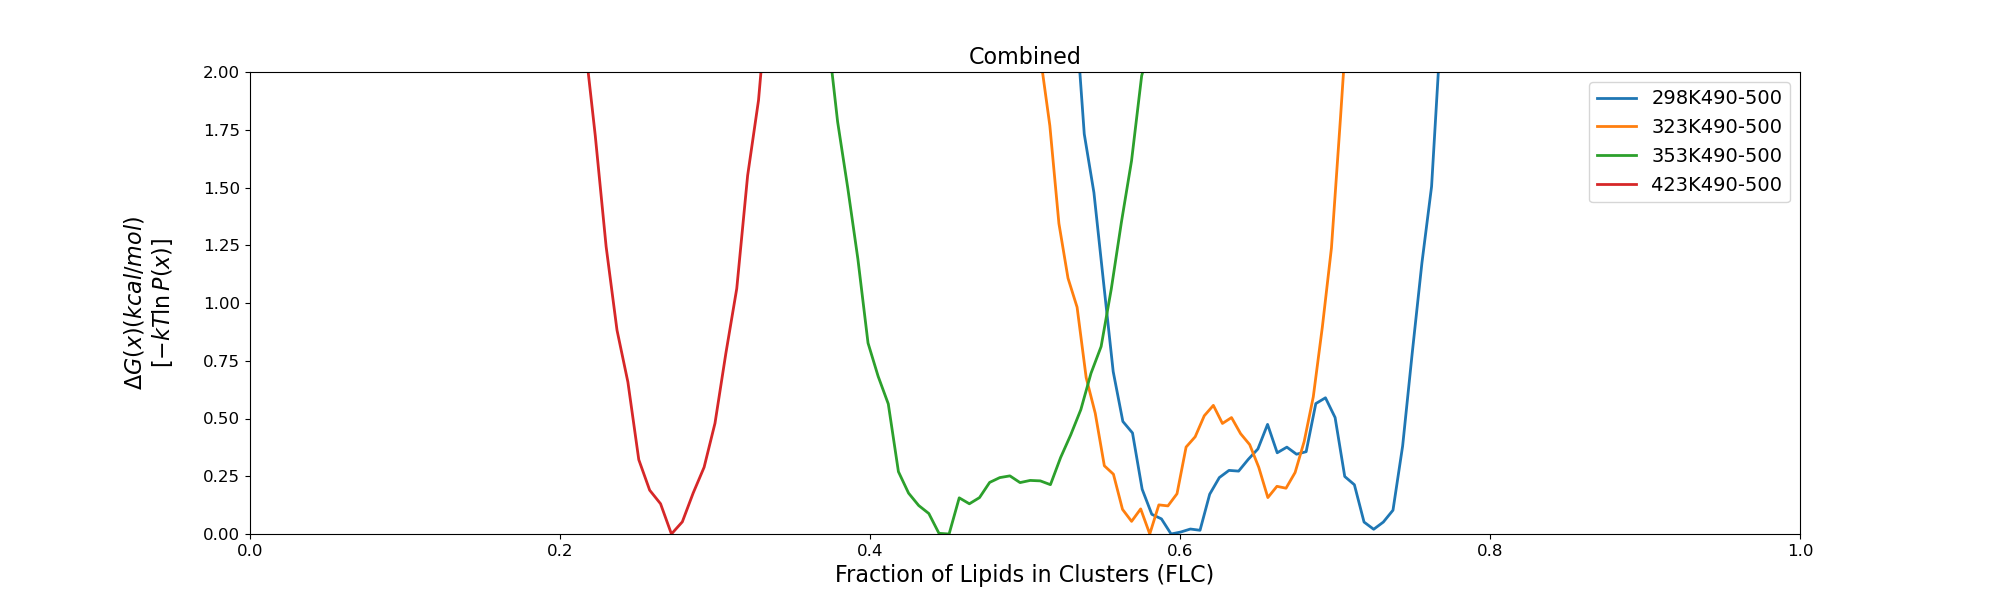
\includegraphics[width=1.1\linewidth]{all_plots/ClusterLipids2Total/DPPC_DIPC_CHOL/Average_DIPC_MULTI__ClusterLipids2Total.png}
\caption{Free Energy Landscape of \textbf{DIPC} system. Data from all four replicas has been combined using w\_multi\_west tool. All the FES are calculated by averaging over the iteration window 490 - 500.}
\label{fig:view}

\end{figure}

\begin{figure}[hbt!]
\centering
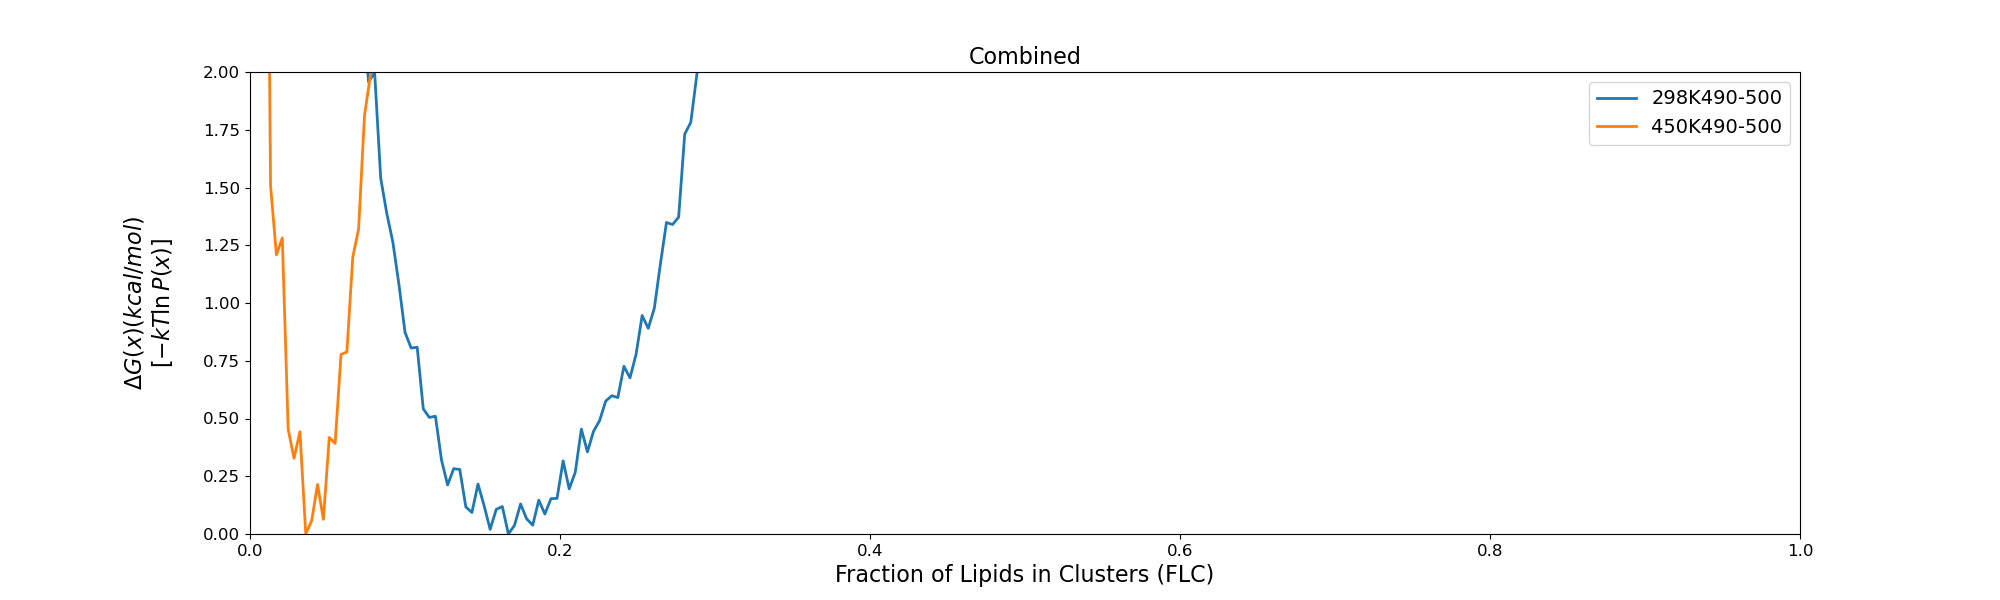
\includegraphics[width=1.1\linewidth]{all_plots/ClusterLipids2Total/DPPC_POPC_CHOL/Average_POPC_MULTI__ClusterLipids2Total.png}
\caption{Free Energy Landscape of \textbf{POPC} system. Data from all four replicas has been combined using w\_multi\_west tool. All the FES are calculated by averaging over the iteration window 490 - 500.}
\label{fig:view}

\end{figure}

\begin{figure}[hbt!]
\centering
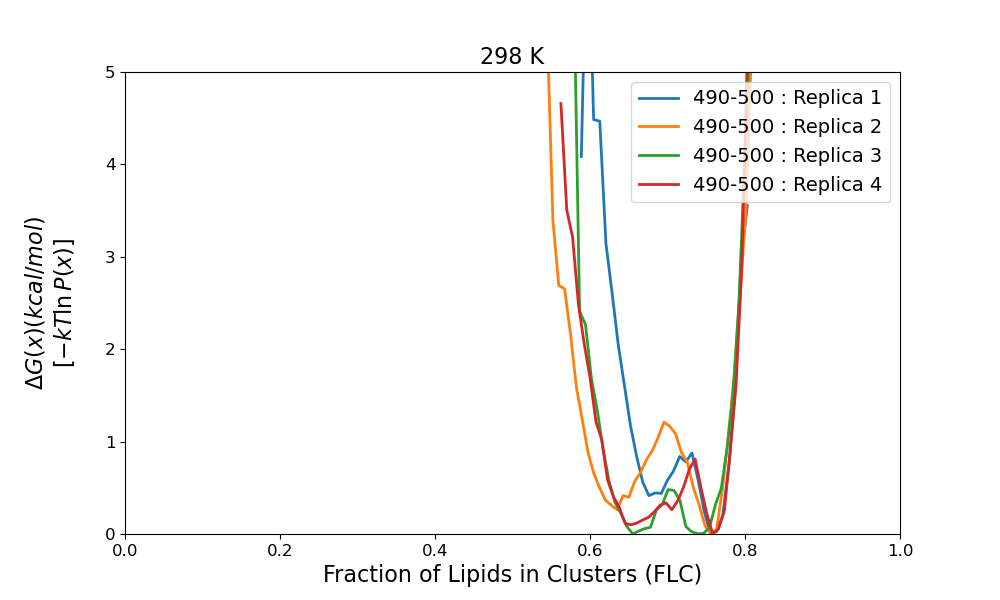
\includegraphics[width=1.1\linewidth]{all_plots/ClusterLipids2Total/DPPC_DAPC_CHOL/298K/Average_DAPC_298_ClusterLipids2Total.png}
\caption{Free Energy Landscape of \textbf{DAPC} system for different replicas at 298K. All the FES are calculated by averaging over the iteration window 490 - 500.}
\label{fig:view}

\end{figure}

\begin{figure}[hbt!]
\centering
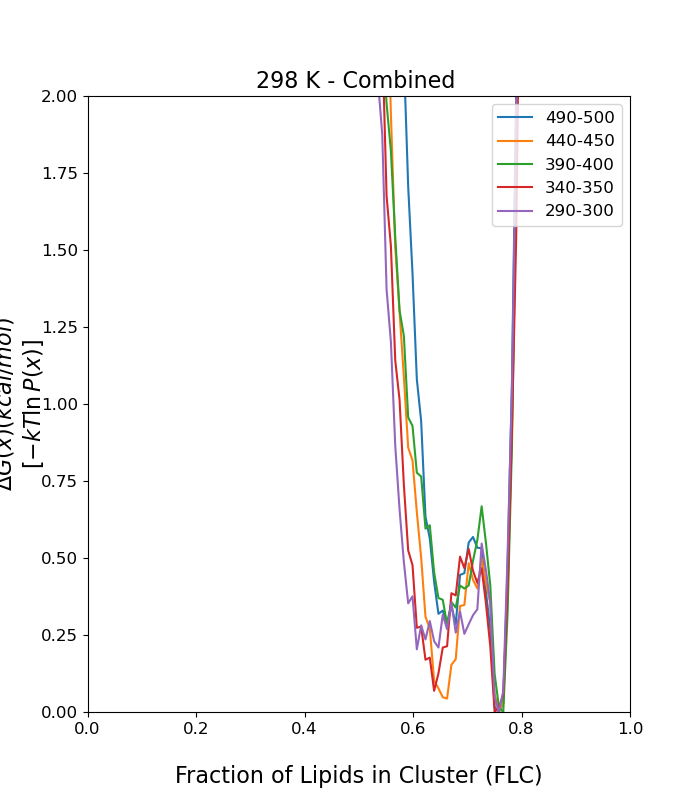
\includegraphics[width=0.6\linewidth]{all_plots/ClusterLipids2Total/DPPC_DAPC_CHOL/298K/Convergence_DAPC_MULTI__298_ClusterLipids2Total.png}
\caption{Convergence of Free Energy Landscape of \textbf{DAPC} system for combined replicas at 298K. All the FES are calculated by averaging over the iteration window 490 - 500.}
\label{fig:view}

\end{figure}

\begin{figure}[hbt!]
\centering
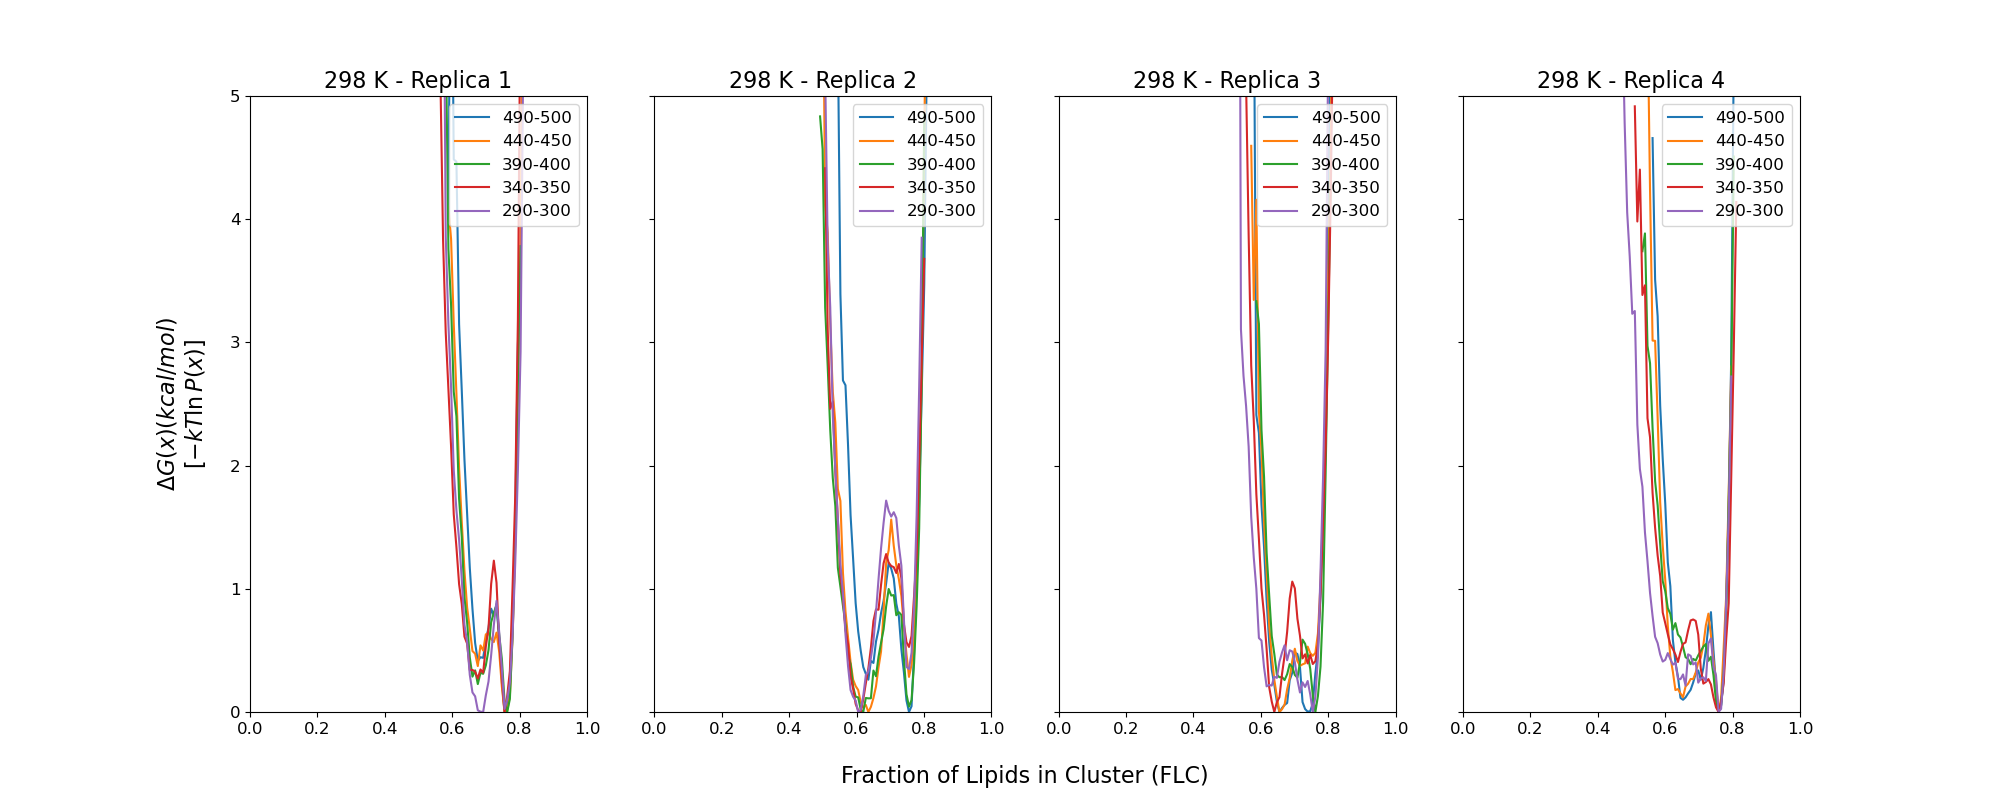
\includegraphics[width=1.1\linewidth]{all_plots/ClusterLipids2Total/DPPC_DAPC_CHOL/298K/Convergence_DAPC_298_ClusterLipids2Total.png}
\caption{Convergence of Free Energy Landscape of \textbf{DAPC} system for different replicas at 298K. All the FES are calculated by averaging over the iteration window 490 - 500.}
\label{fig:view}

\end{figure}

\begin{figure}[hbt!]
\centering
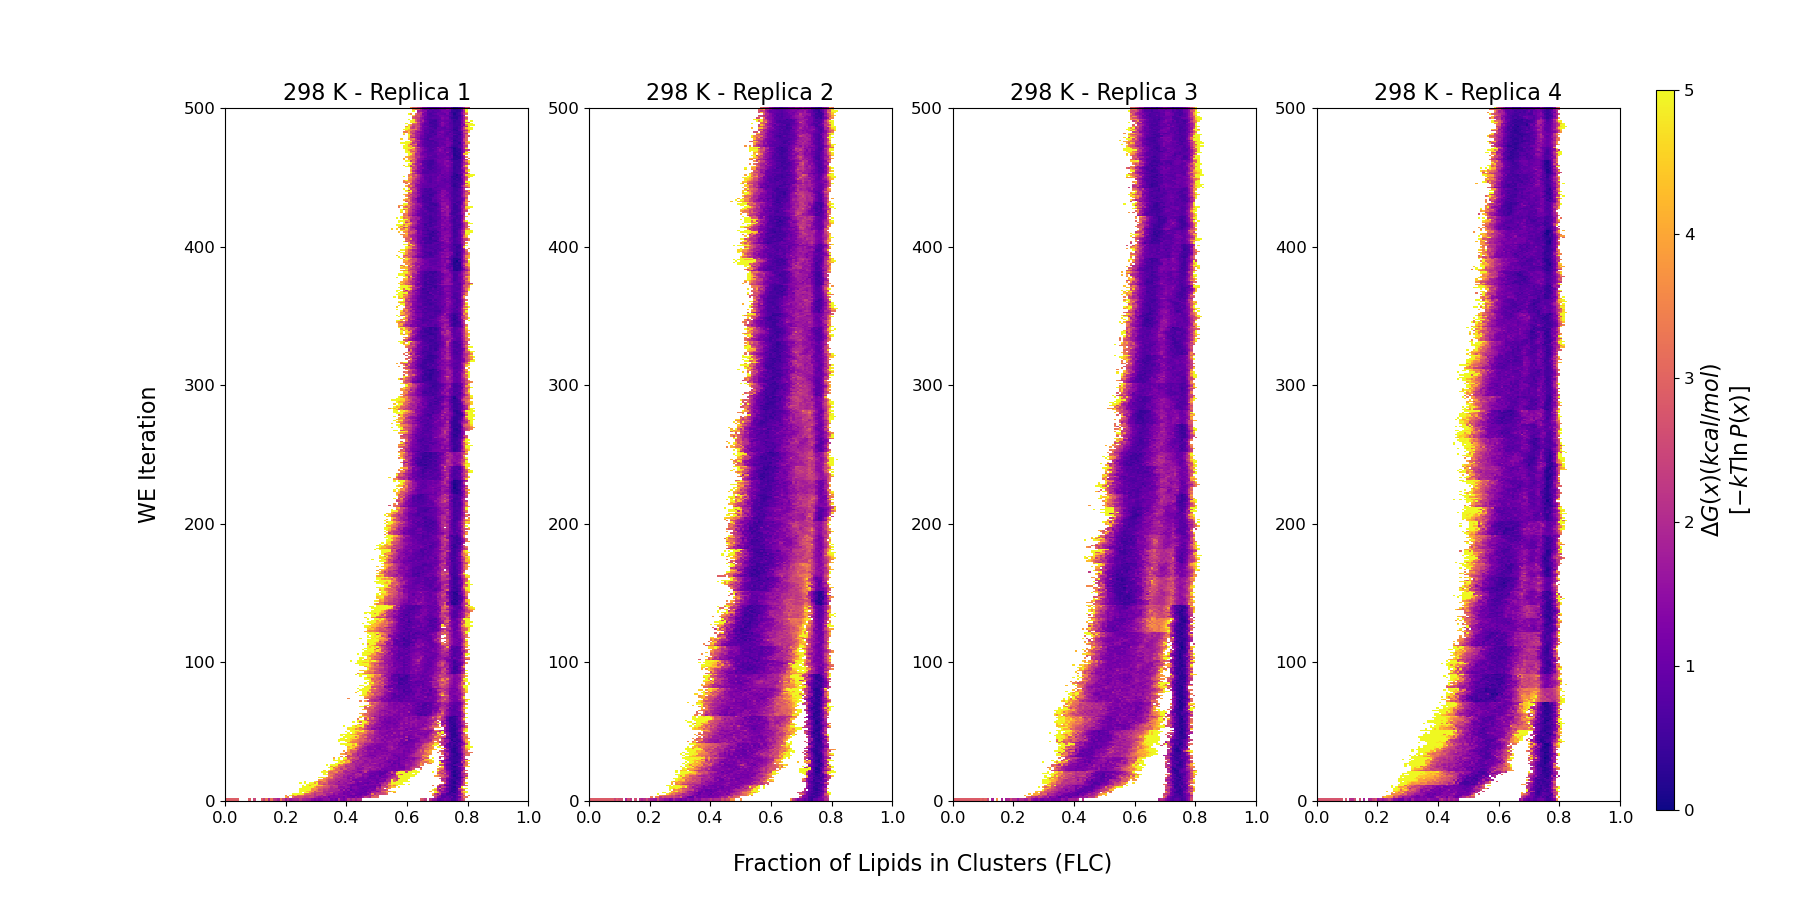
\includegraphics[width=1.1\linewidth]{all_plots/ClusterLipids2Total/DPPC_DAPC_CHOL/298K/Evolution_DAPC_298_ClusterLipids2Total.png}
\caption{Evolution of Free Energy Landscape of \textbf{DAPC} system for different replicas at 298K.}
\label{fig:view}

\end{figure}

\begin{figure}[hbt!]
\centering
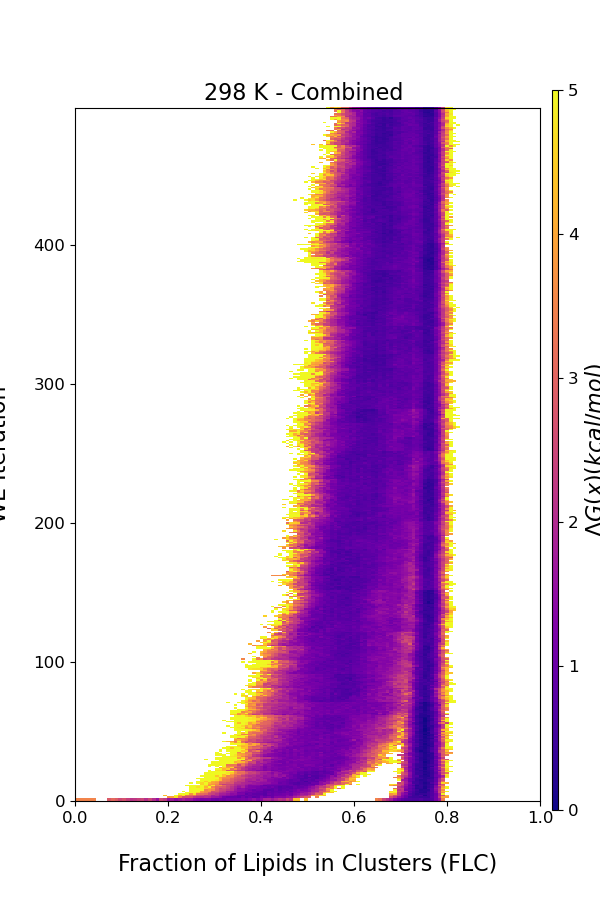
\includegraphics[width=0.8\linewidth]{all_plots/ClusterLipids2Total/DPPC_DAPC_CHOL/298K/Evolution_DAPC_MULTI__298_ClusterLipids2Total.png}
\caption{Evolution of Free Energy Landscape of \textbf{DAPC} system for combined replicas at 298K using w\_multi\_tool.}
\label{fig:view}

\end{figure}

%----------------------------%

\begin{figure}[hbt!]
\centering
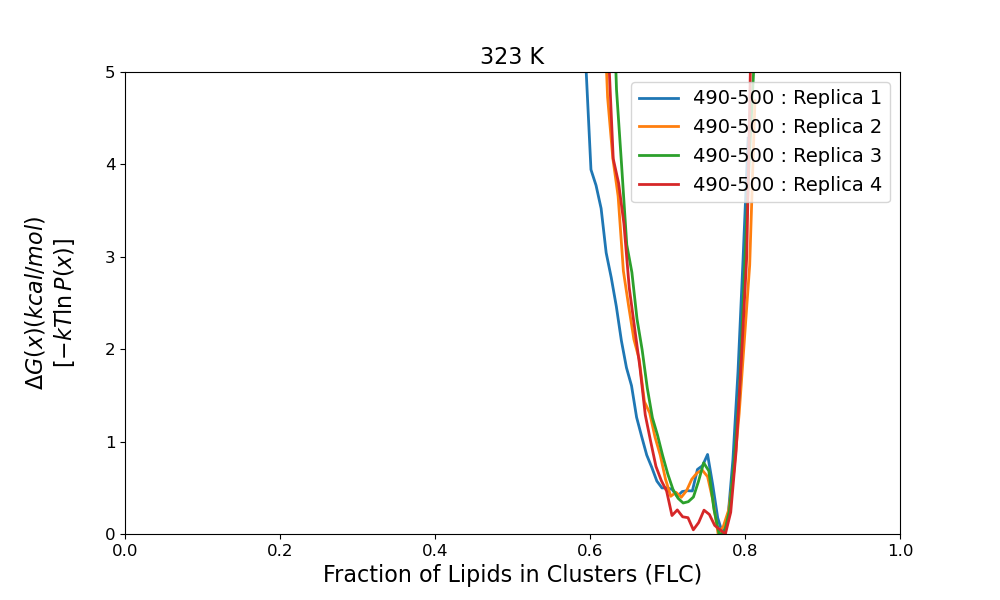
\includegraphics[width=1.1\linewidth]{all_plots/ClusterLipids2Total/DPPC_DAPC_CHOL/323K/Average_DAPC_323_ClusterLipids2Total.png}
\caption{Free Energy Landscape of \textbf{DAPC} system for different replicas at 323K. All the FES are calculated by averaging over the iteration window 490 - 500.}
\label{fig:view}

\end{figure}

\begin{figure}[hbt!]
\centering
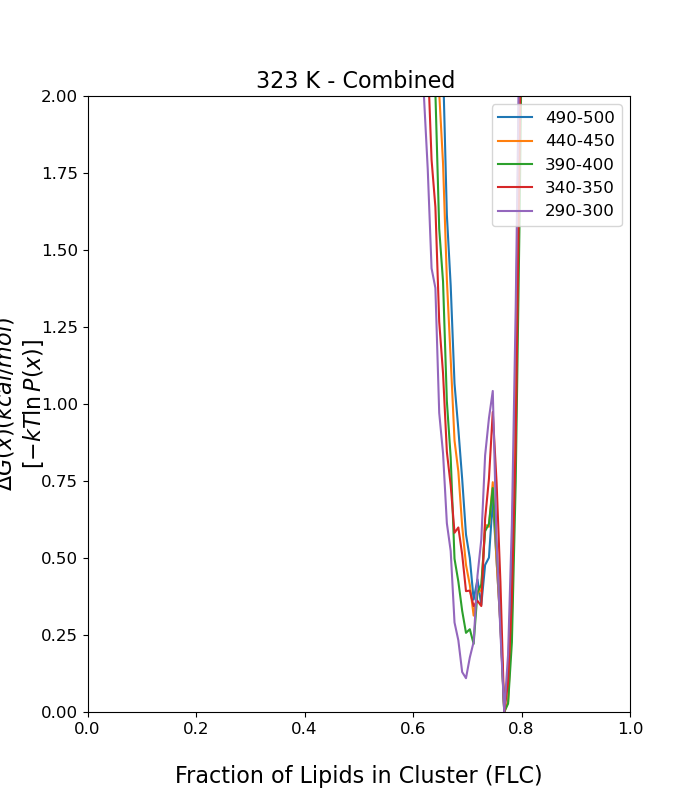
\includegraphics[width=0.6\linewidth]{all_plots/ClusterLipids2Total/DPPC_DAPC_CHOL/323K/Convergence_DAPC_MULTI__323_ClusterLipids2Total.png}
\caption{Convergence of Free Energy Landscape of \textbf{DAPC} system for combined replicas at 323K. All the FES are calculated by averaging over the iteration window 490 - 500.}
\label{fig:view}

\end{figure}

\begin{figure}[hbt!]
\centering
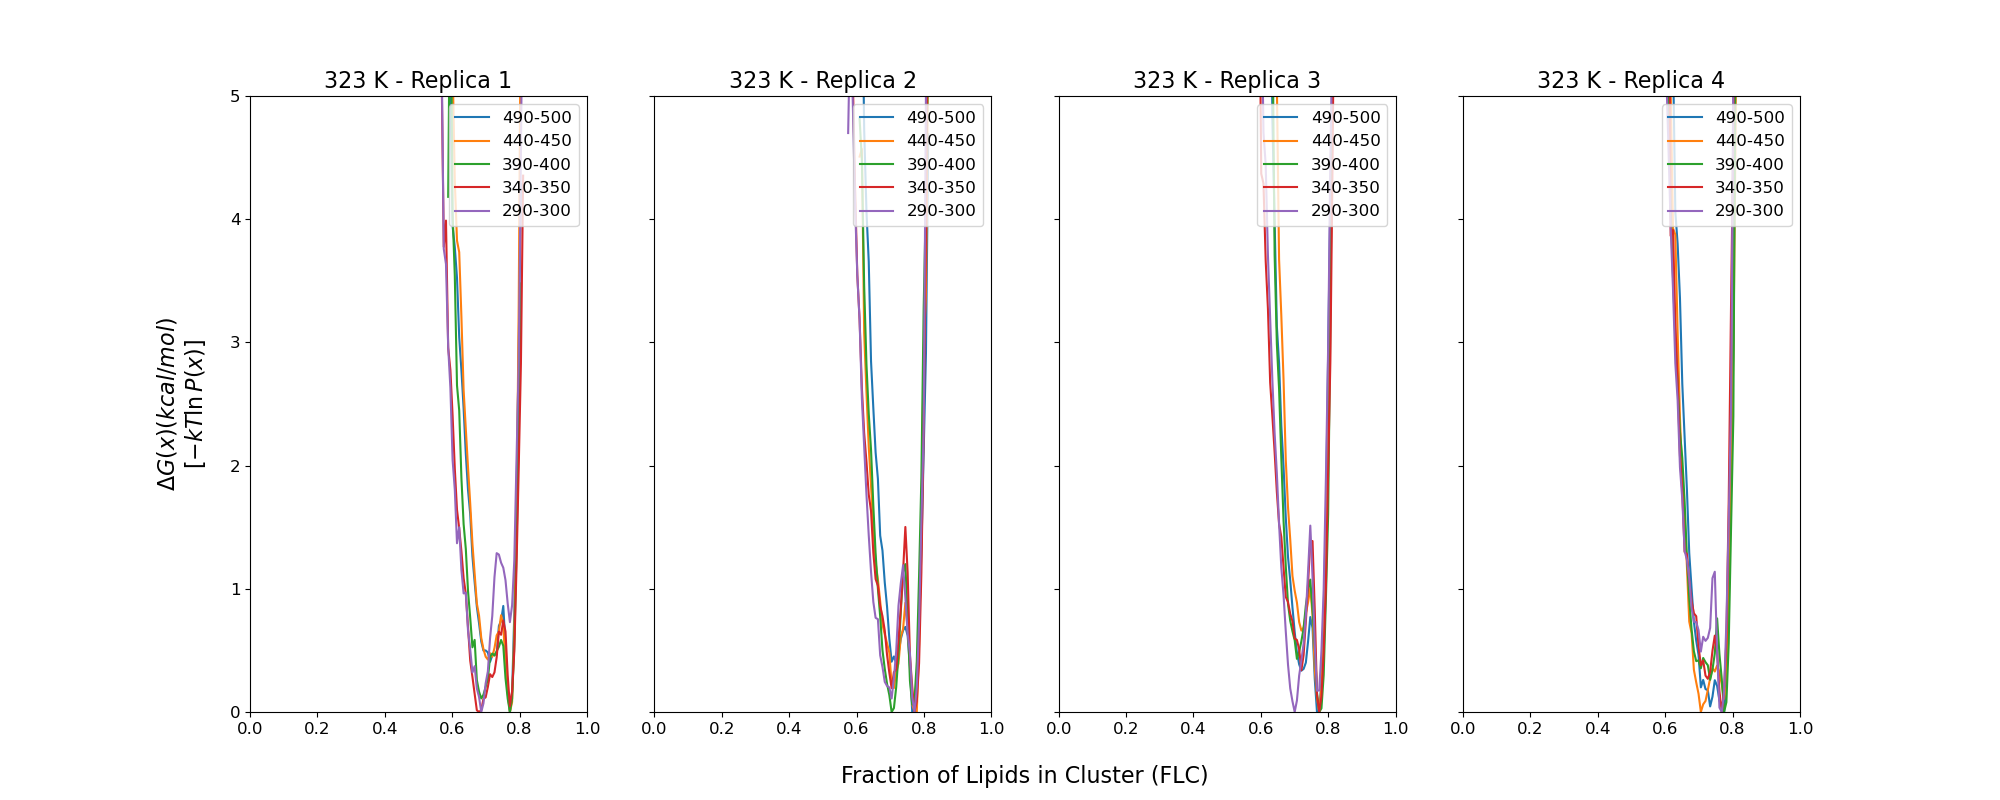
\includegraphics[width=1.1\linewidth]{all_plots/ClusterLipids2Total/DPPC_DAPC_CHOL/323K/Convergence_DAPC_323_ClusterLipids2Total.png}
\caption{Convergence of Free Energy Landscape of \textbf{DAPC} system for different replicas at 323K. All the FES are calculated by averaging over the iteration window 490 - 500.}
\label{fig:view}

\end{figure}

\begin{figure}[hbt!]
\centering
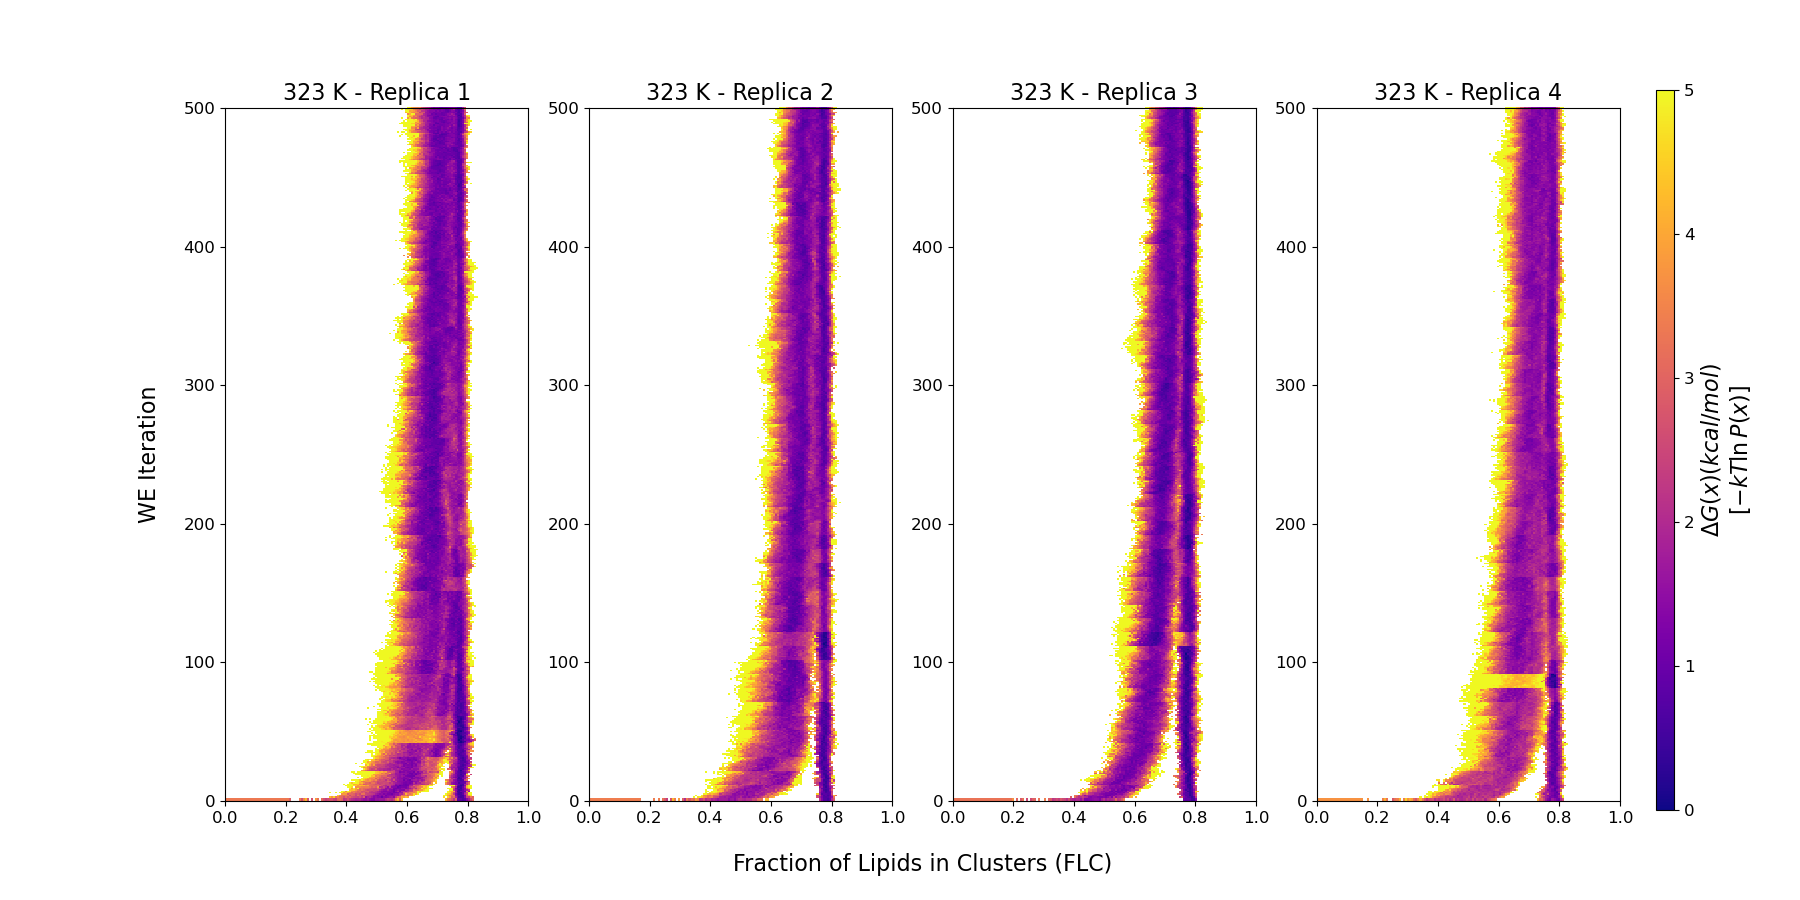
\includegraphics[width=1.1\linewidth]{all_plots/ClusterLipids2Total/DPPC_DAPC_CHOL/323K/Evolution_DAPC_323_ClusterLipids2Total.png}
\caption{Evolution of Free Energy Landscape of \textbf{DAPC} system for different replicas at 323K.}
\label{fig:view}

\end{figure}

\begin{figure}[hbt!]
\centering
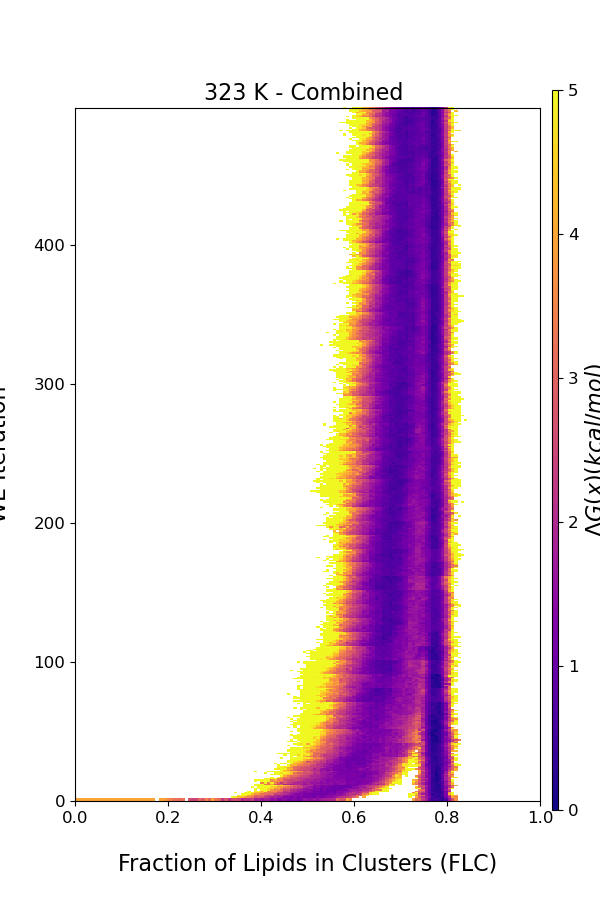
\includegraphics[width=0.8\linewidth]{all_plots/ClusterLipids2Total/DPPC_DAPC_CHOL/323K/Evolution_DAPC_MULTI__323_ClusterLipids2Total.png}
\caption{Evolution of Free Energy Landscape of \textbf{DAPC} system for combined replicas at 323K using w\_multi\_tool.}
\label{fig:view}

\end{figure}

%---------------------%

\begin{figure}[hbt!]
\centering
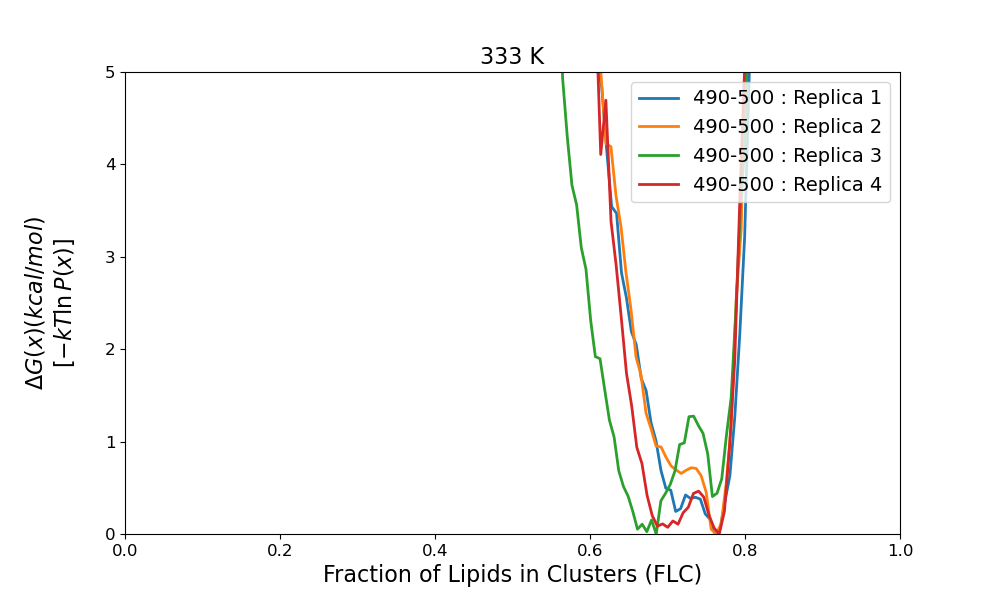
\includegraphics[width=1.1\linewidth]{all_plots/ClusterLipids2Total/DPPC_DAPC_CHOL/333K/Average_DAPC_333_ClusterLipids2Total.png}
\caption{Free Energy Landscape of \textbf{DAPC} system for different replicas at 333K. All the FES are calculated by averaging over the iteration window 490 - 500.}
\label{fig:view}

\end{figure}

\begin{figure}[hbt!]
\centering
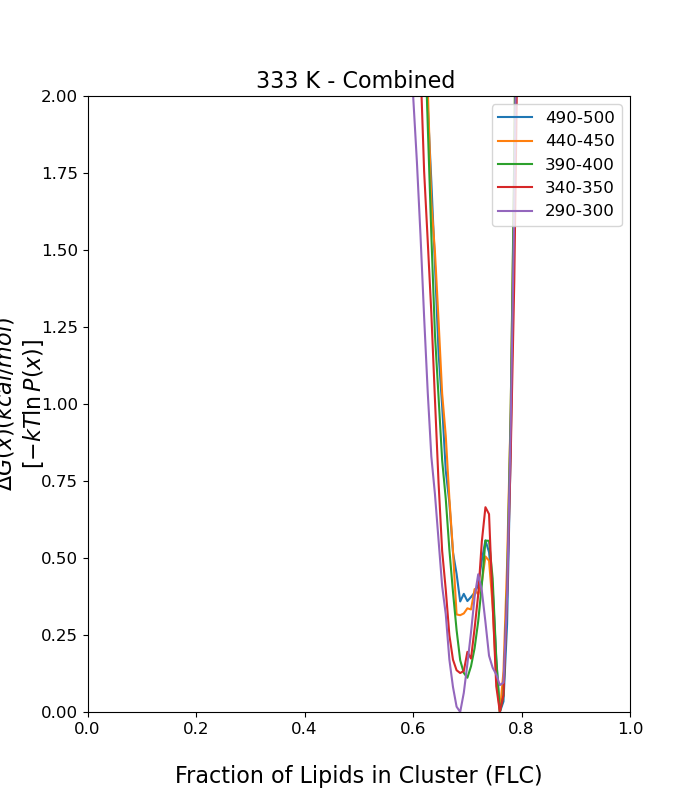
\includegraphics[width=0.6\linewidth]{all_plots/ClusterLipids2Total/DPPC_DAPC_CHOL/333K/Convergence_DAPC_MULTI__333_ClusterLipids2Total.png}
\caption{Convergence of Free Energy Landscape of \textbf{DAPC} system for combined replicas at 333K. All the FES are calculated by averaging over the iteration window 490 - 500.}
\label{fig:view}

\end{figure}

\begin{figure}[hbt!]
\centering
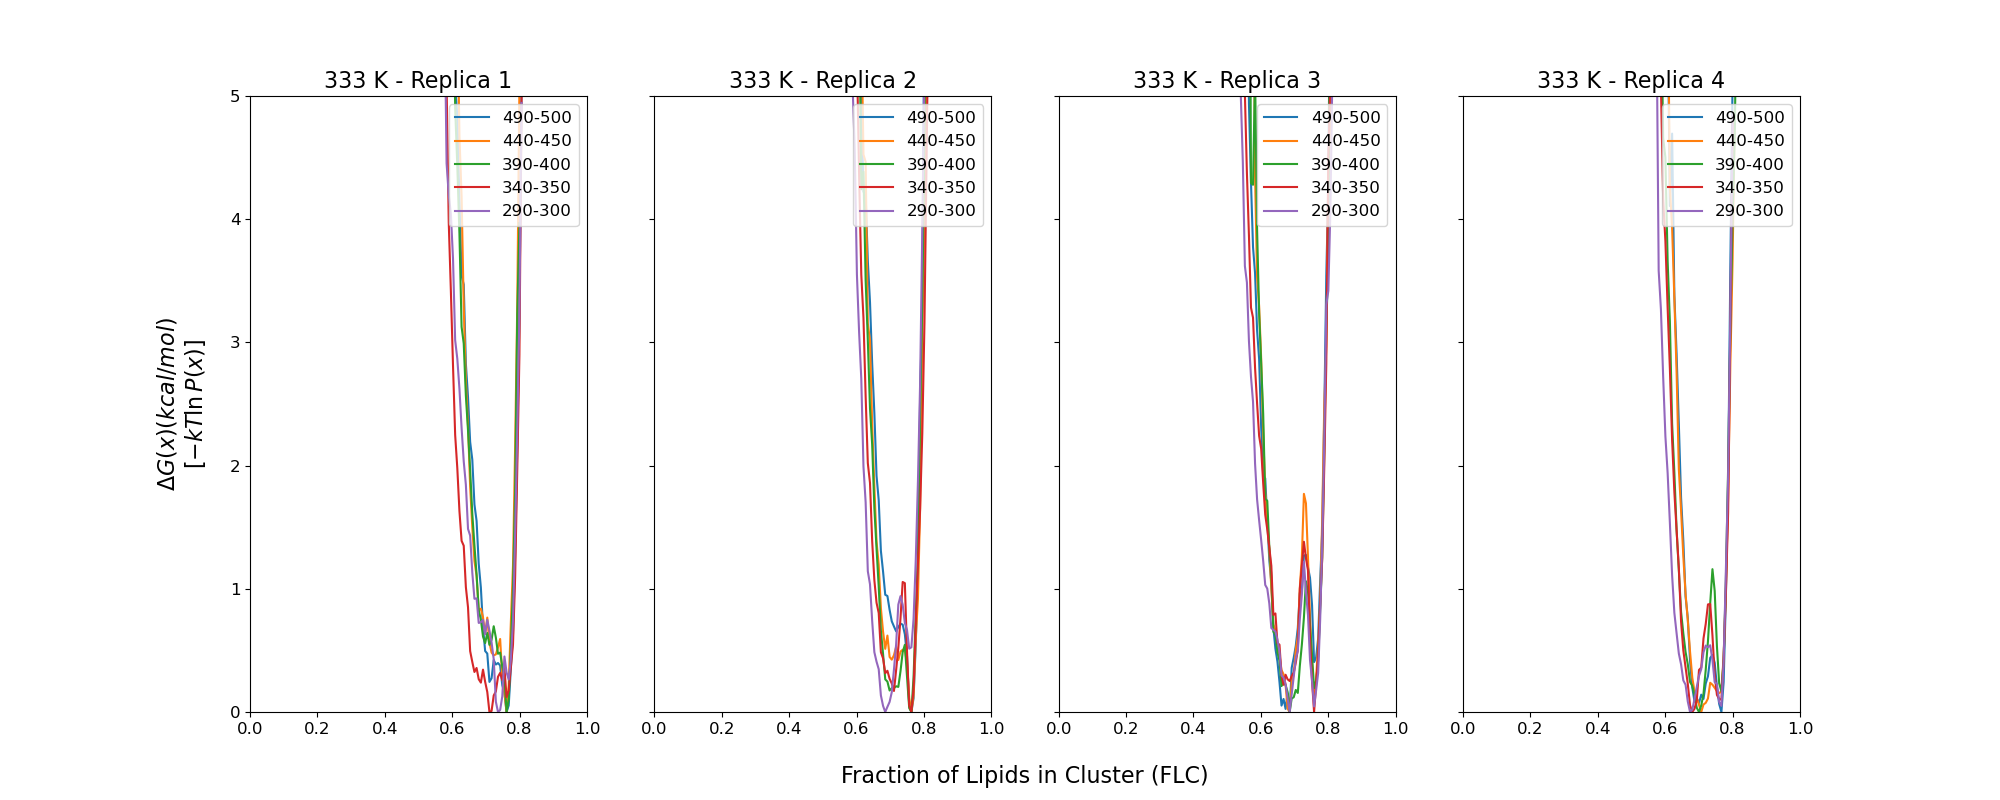
\includegraphics[width=1.1\linewidth]{all_plots/ClusterLipids2Total/DPPC_DAPC_CHOL/333K/Convergence_DAPC_333_ClusterLipids2Total.png}
\caption{Convergence of Free Energy Landscape of \textbf{DAPC} system for different replicas at 333K. All the FES are calculated by averaging over the iteration window 490 - 500.}
\label{fig:view}

\end{figure}

\begin{figure}[hbt!]
\centering
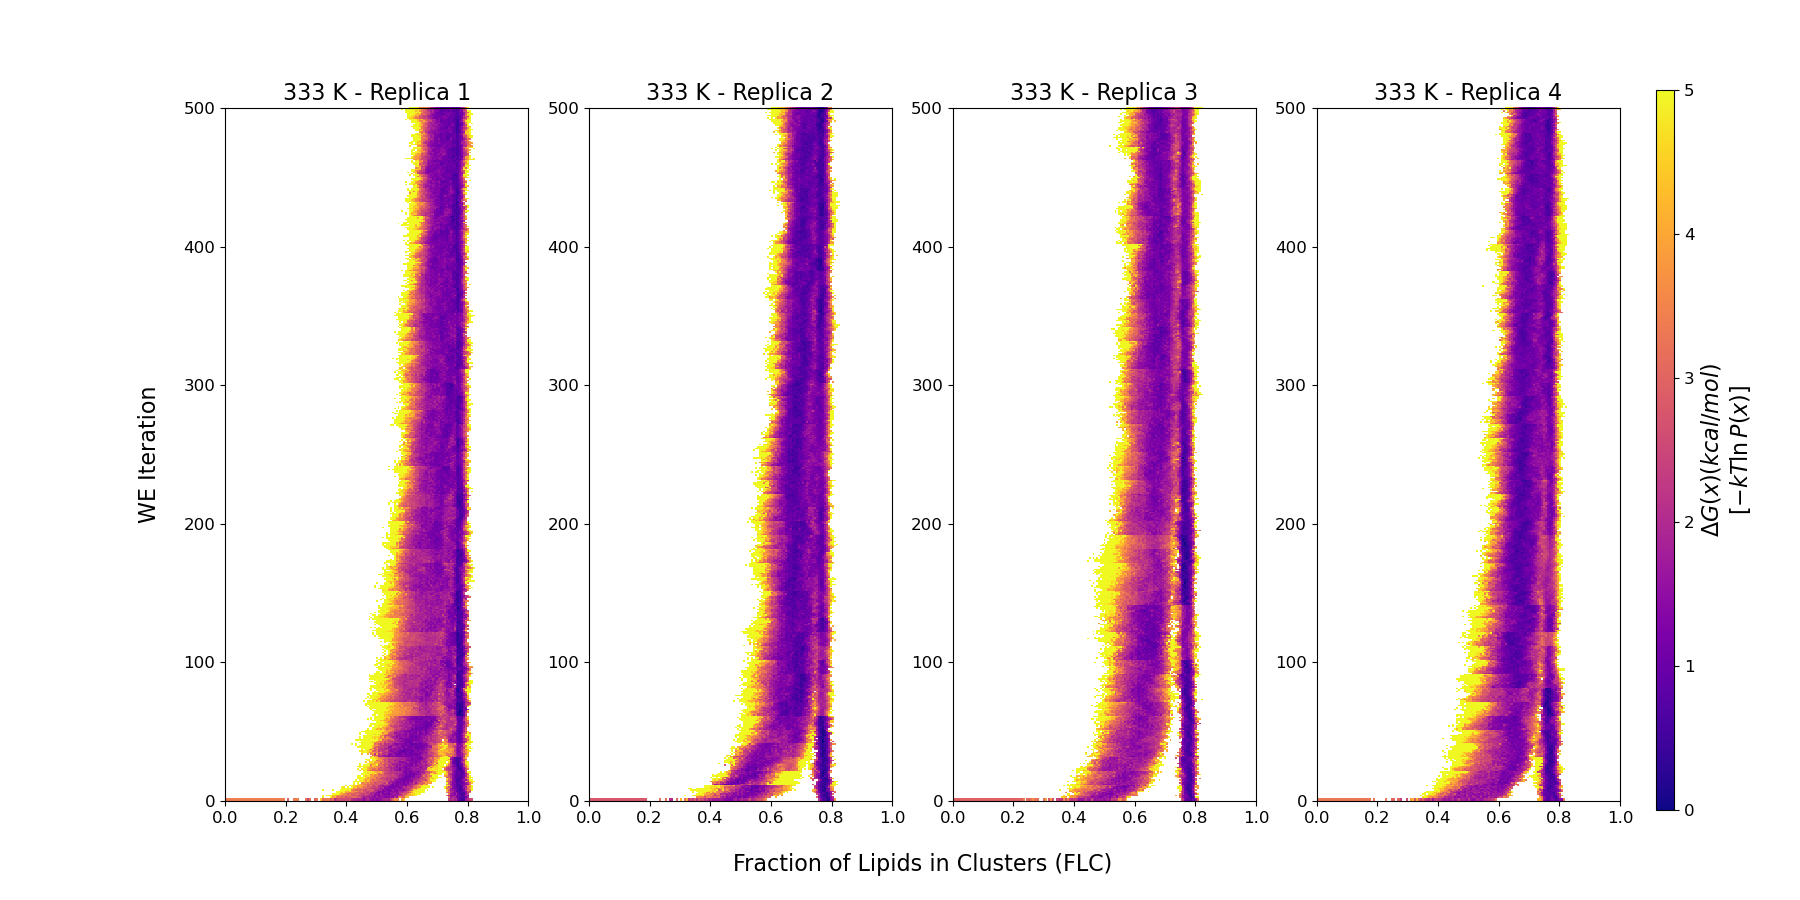
\includegraphics[width=1.1\linewidth]{all_plots/ClusterLipids2Total/DPPC_DAPC_CHOL/333K/Evolution_DAPC_333_ClusterLipids2Total.png}
\caption{Evolution of Free Energy Landscape of \textbf{DAPC} system for different replicas at 333K.}
\label{fig:view}

\end{figure}

\begin{figure}[hbt!]
\centering
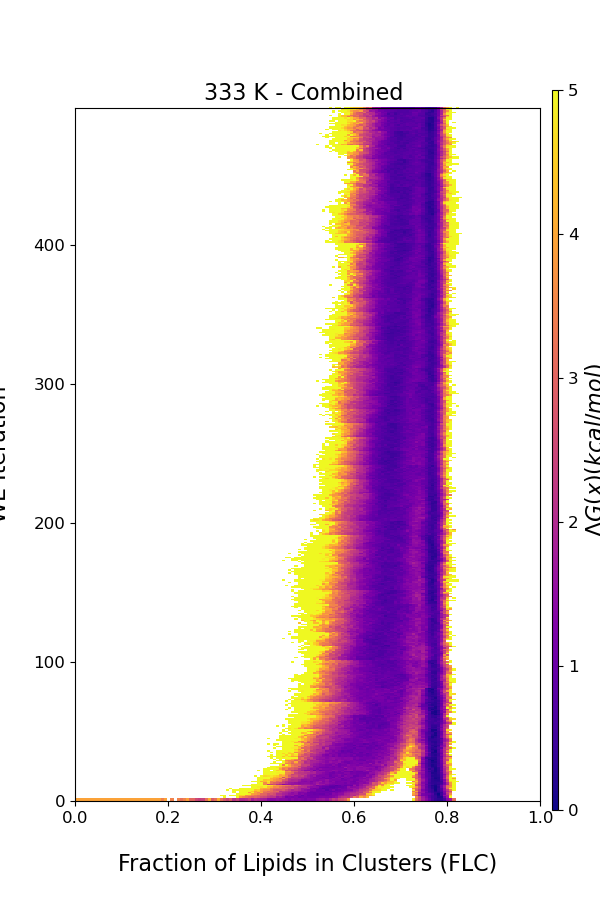
\includegraphics[width=0.8\linewidth]{all_plots/ClusterLipids2Total/DPPC_DAPC_CHOL/333K/Evolution_DAPC_MULTI__333_ClusterLipids2Total.png}
\caption{Evolution of Free Energy Landscape of \textbf{DAPC} system for combined replicas at 333K using w\_multi\_tool.}
\label{fig:view}

\end{figure}

%---------------------%

\begin{figure}[hbt!]
\centering
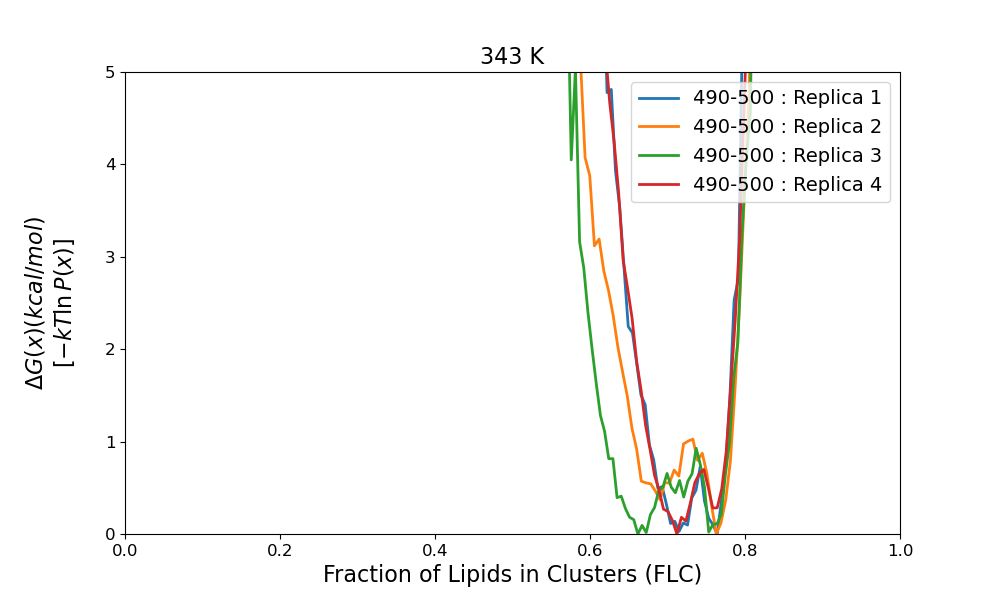
\includegraphics[width=1.1\linewidth]{all_plots/ClusterLipids2Total/DPPC_DAPC_CHOL/343K/Average_DAPC_343_ClusterLipids2Total.png}
\caption{Free Energy Landscape of \textbf{DAPC} system for different replicas at 343K. All the FES are calculated by averaging over the iteration window 490 - 500.}
\label{fig:view}

\end{figure}

\begin{figure}[hbt!]
\centering
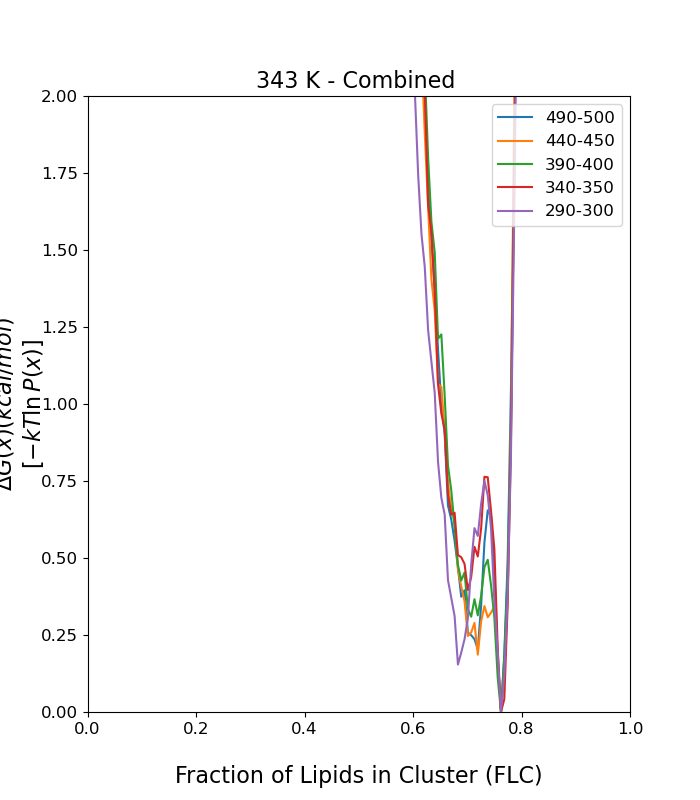
\includegraphics[width=0.6\linewidth]{all_plots/ClusterLipids2Total/DPPC_DAPC_CHOL/343K/Convergence_DAPC_MULTI__343_ClusterLipids2Total.png}
\caption{Convergence of Free Energy Landscape of \textbf{DAPC} system for combined replicas at 343K. All the FES are calculated by averaging over the iteration window 490 - 500.}
\label{fig:view}

\end{figure}

\begin{figure}[hbt!]
\centering
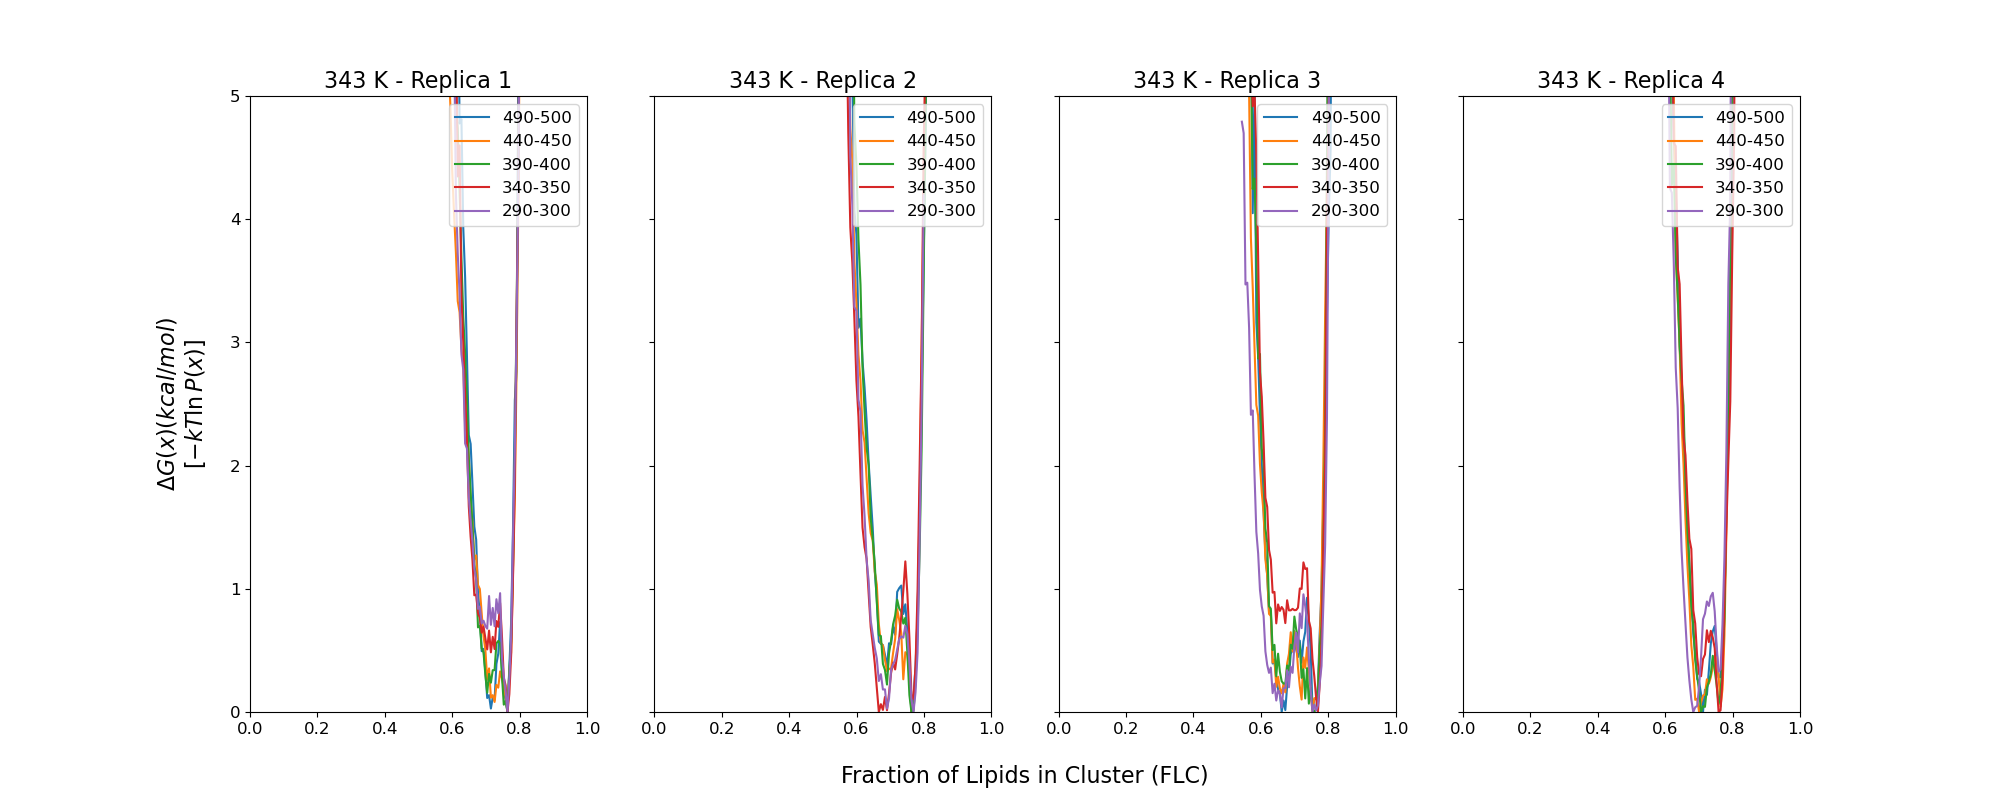
\includegraphics[width=1.1\linewidth]{all_plots/ClusterLipids2Total/DPPC_DAPC_CHOL/343K/Convergence_DAPC_343_ClusterLipids2Total.png}
\caption{Convergence of Free Energy Landscape of \textbf{DAPC} system for different replicas at 343K. All the FES are calculated by averaging over the iteration window 490 - 500.}
\label{fig:view}

\end{figure}

\begin{figure}[hbt!]
\centering
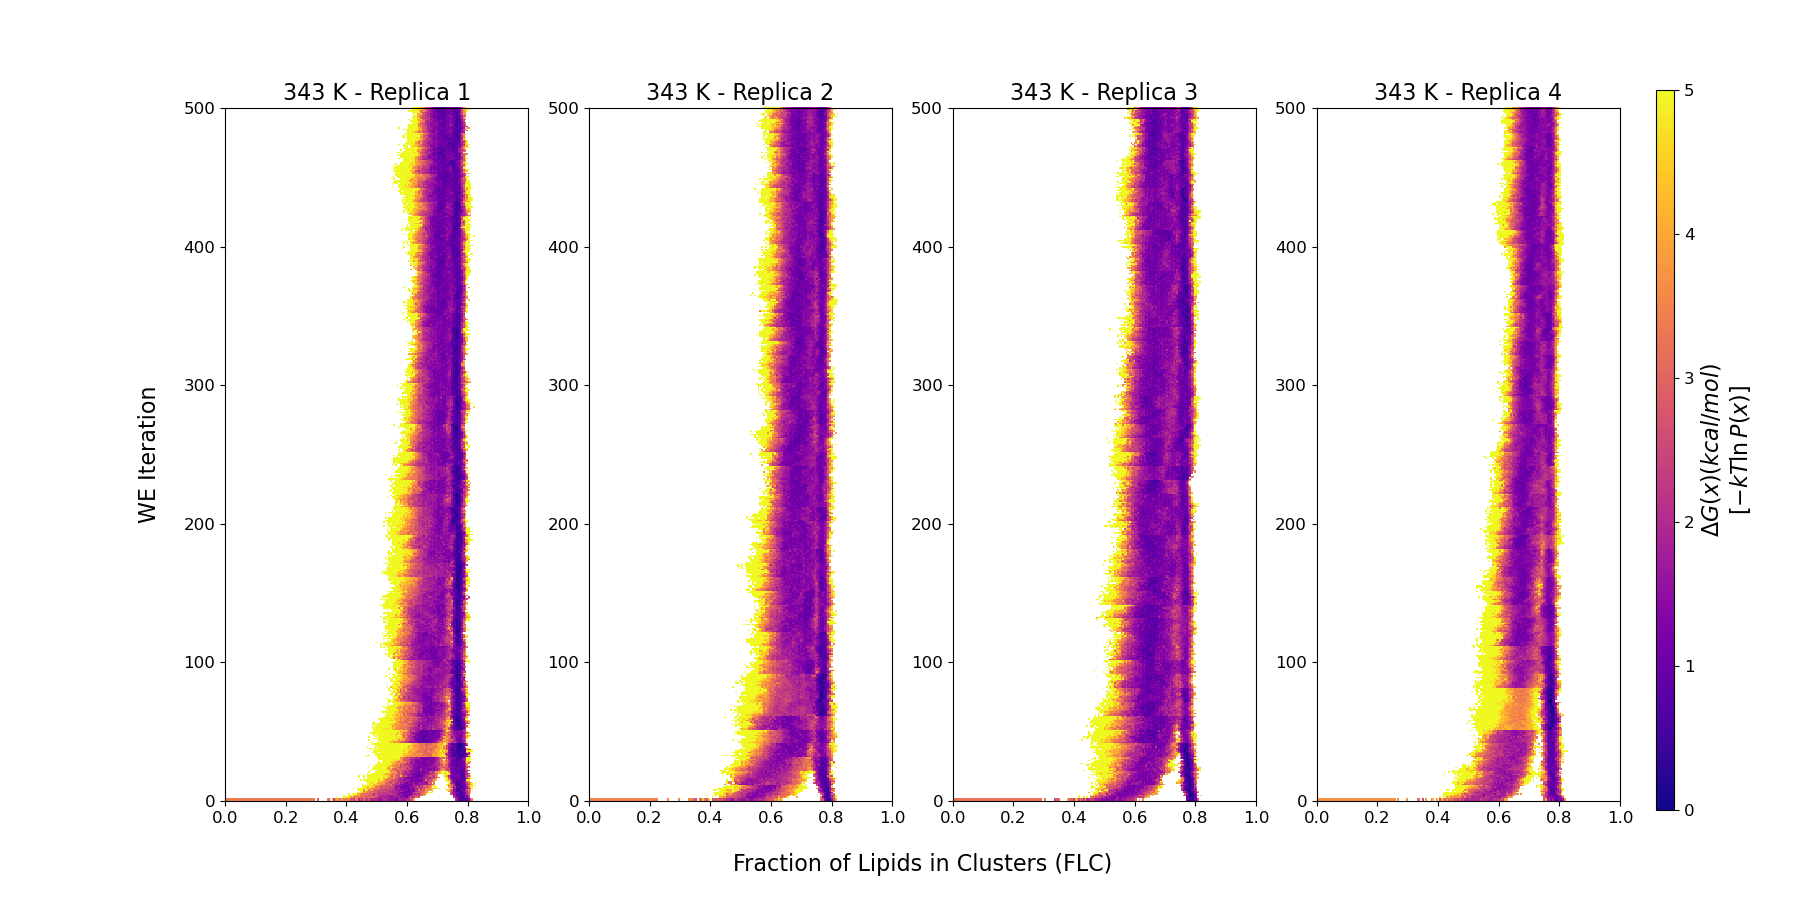
\includegraphics[width=1.1\linewidth]{all_plots/ClusterLipids2Total/DPPC_DAPC_CHOL/343K/Evolution_DAPC_343_ClusterLipids2Total.png}
\caption{Evolution of Free Energy Landscape of \textbf{DAPC} system for different replicas at 343K.}
\label{fig:view}

\end{figure}

\begin{figure}[hbt!]
\centering
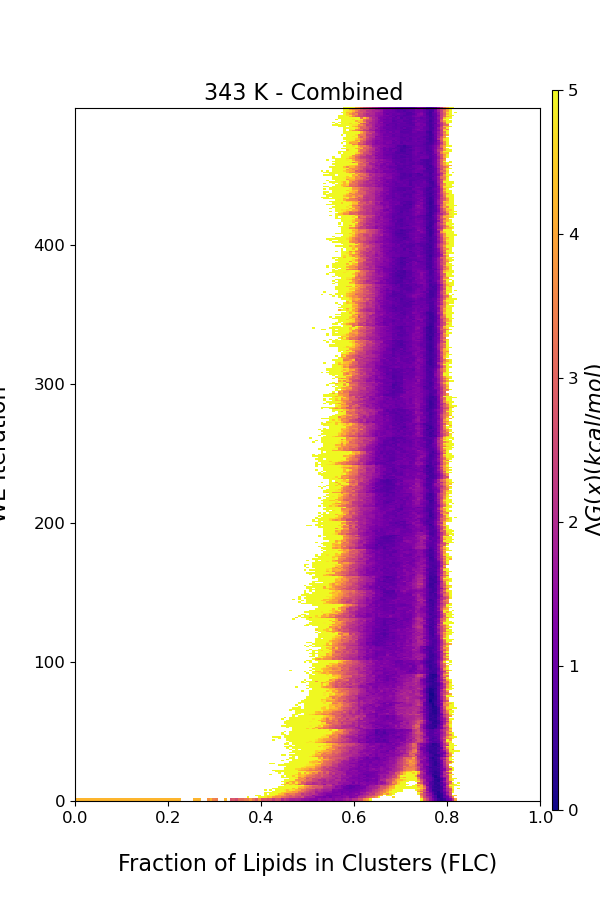
\includegraphics[width=0.8\linewidth]{all_plots/ClusterLipids2Total/DPPC_DAPC_CHOL/343K/Evolution_DAPC_MULTI__343_ClusterLipids2Total.png}
\caption{Evolution of Free Energy Landscape of \textbf{DAPC} system for combined replicas at 343K using w\_multi\_tool.}
\label{fig:view}

\end{figure}

%---------------------%

\begin{figure}[hbt!]
\centering
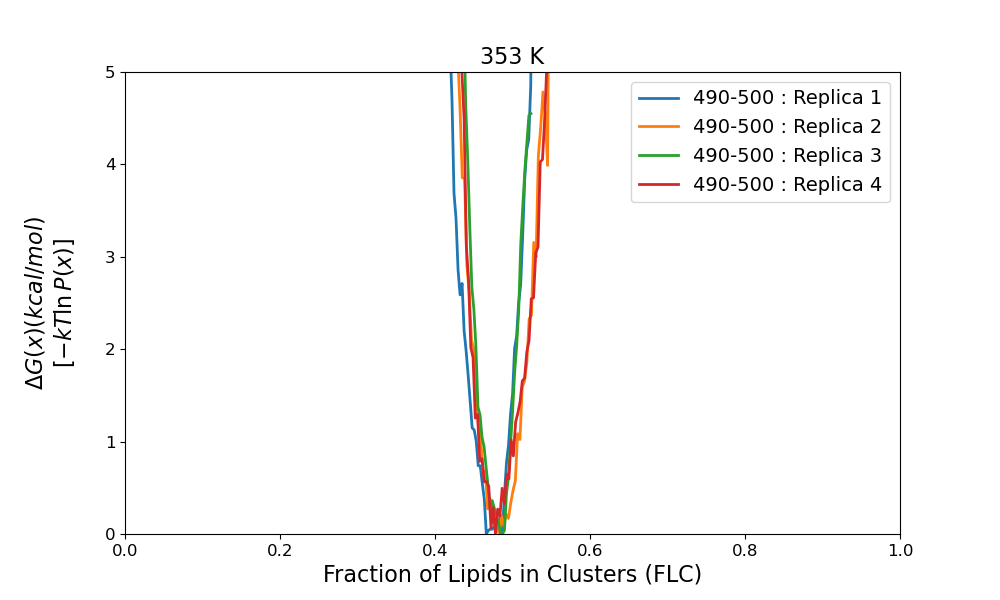
\includegraphics[width=1.1\linewidth]{all_plots/ClusterLipids2Total/DPPC_DAPC_CHOL/353K/Average_DAPC_353_ClusterLipids2Total.png}
\caption{Free Energy Landscape of \textbf{DAPC} system for different replicas at 353K. All the FES are calculated by averaging over the iteration window 490 - 500.}
\label{fig:view}

\end{figure}

\begin{figure}[hbt!]
\centering
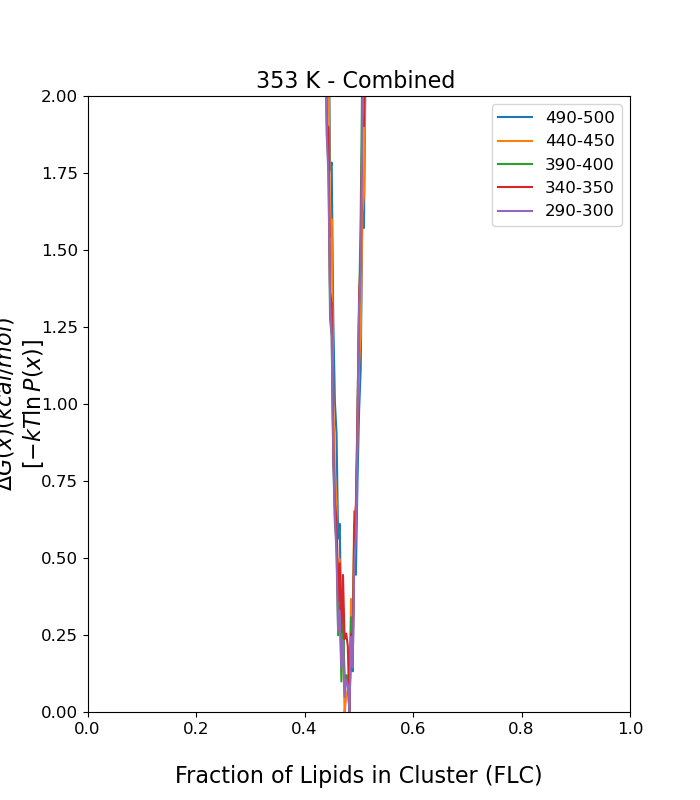
\includegraphics[width=0.6\linewidth]{all_plots/ClusterLipids2Total/DPPC_DAPC_CHOL/353K/Convergence_DAPC_MULTI__353_ClusterLipids2Total.png}
\caption{Convergence of Free Energy Landscape of \textbf{DAPC} system for combined replicas at 353K. All the FES are calculated by averaging over the iteration window 490 - 500.}
\label{fig:view}

\end{figure}

\begin{figure}[hbt!]
\centering
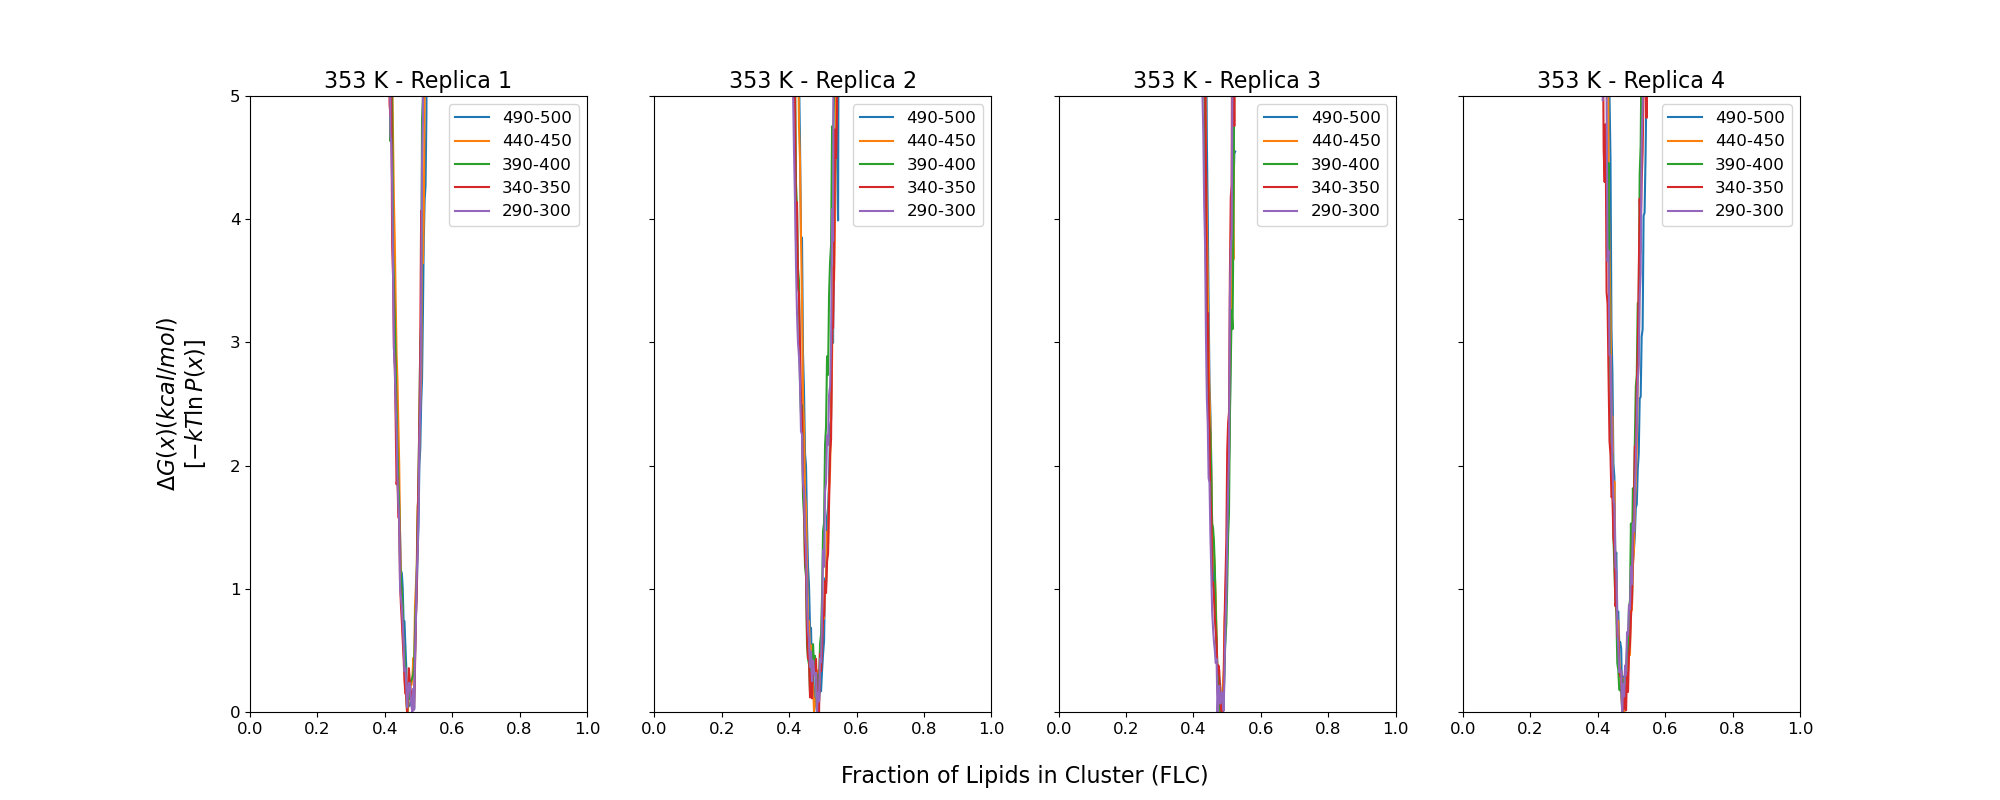
\includegraphics[width=1.1\linewidth]{all_plots/ClusterLipids2Total/DPPC_DAPC_CHOL/353K/Convergence_DAPC_353_ClusterLipids2Total.png}
\caption{Convergence of Free Energy Landscape of \textbf{DAPC} system for different replicas at 353K. All the FES are calculated by averaging over the iteration window 490 - 500.}
\label{fig:view}

\end{figure}

\begin{figure}[hbt!]
\centering
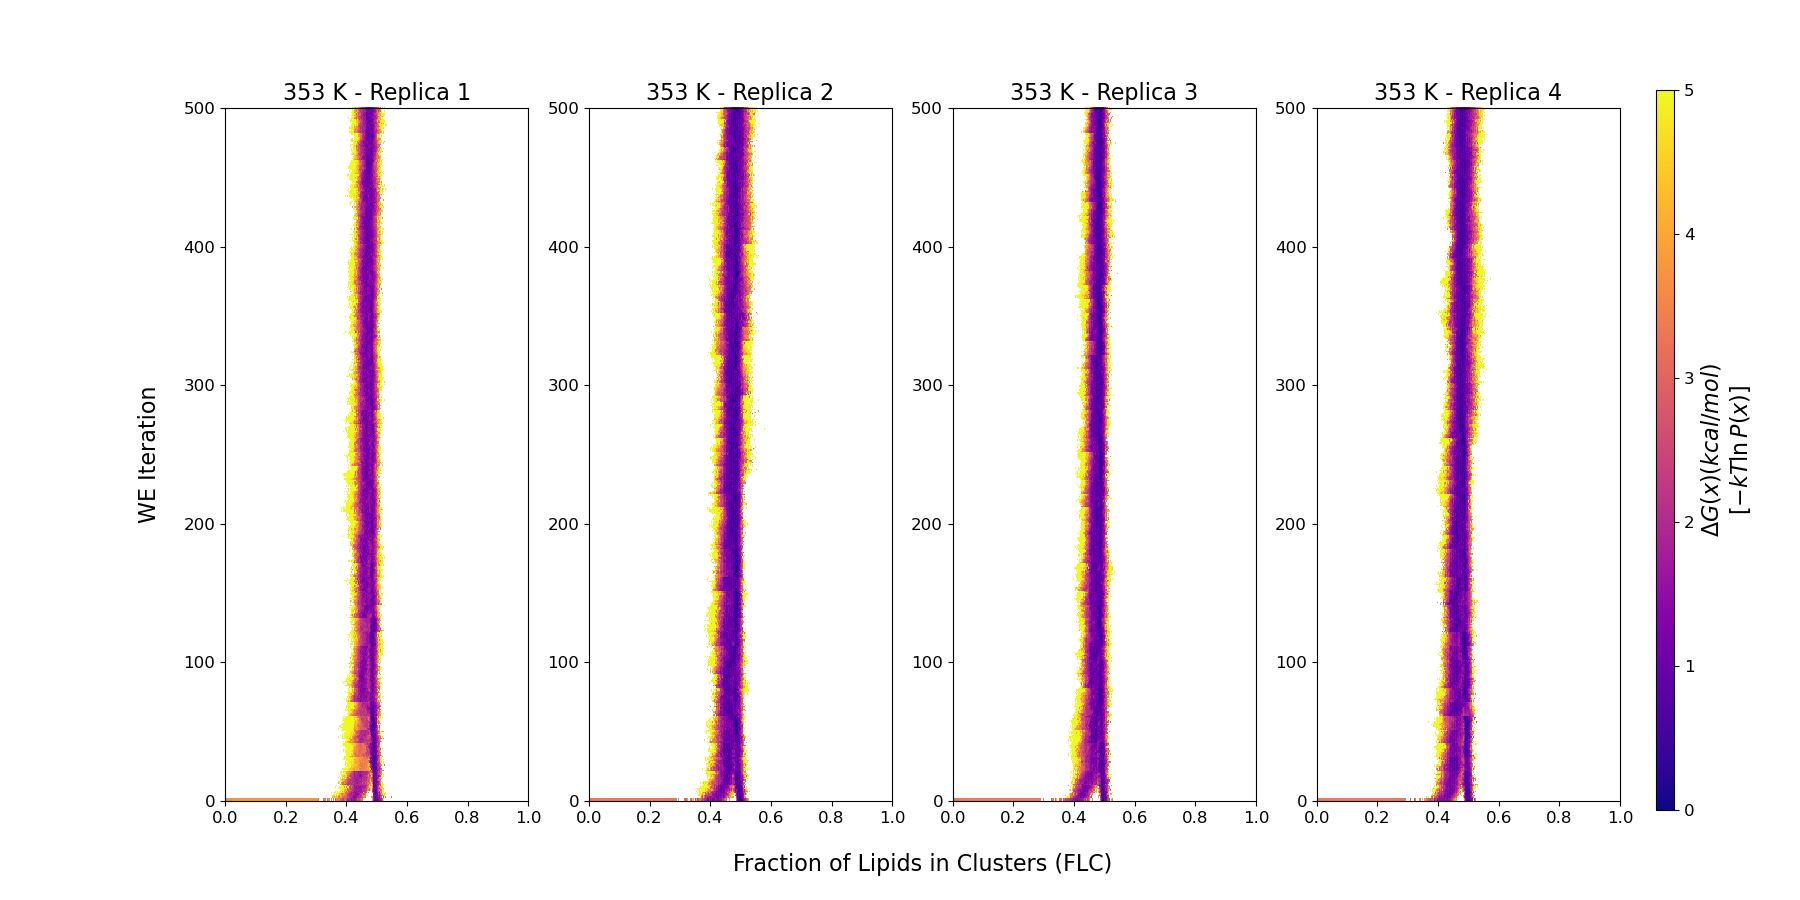
\includegraphics[width=1.1\linewidth]{all_plots/ClusterLipids2Total/DPPC_DAPC_CHOL/353K/Evolution_DAPC_353_ClusterLipids2Total.png}
\caption{Evolution of Free Energy Landscape of \textbf{DAPC} system for different replicas at 353K.}
\label{fig:view}

\end{figure}

\begin{figure}[hbt!]
\centering
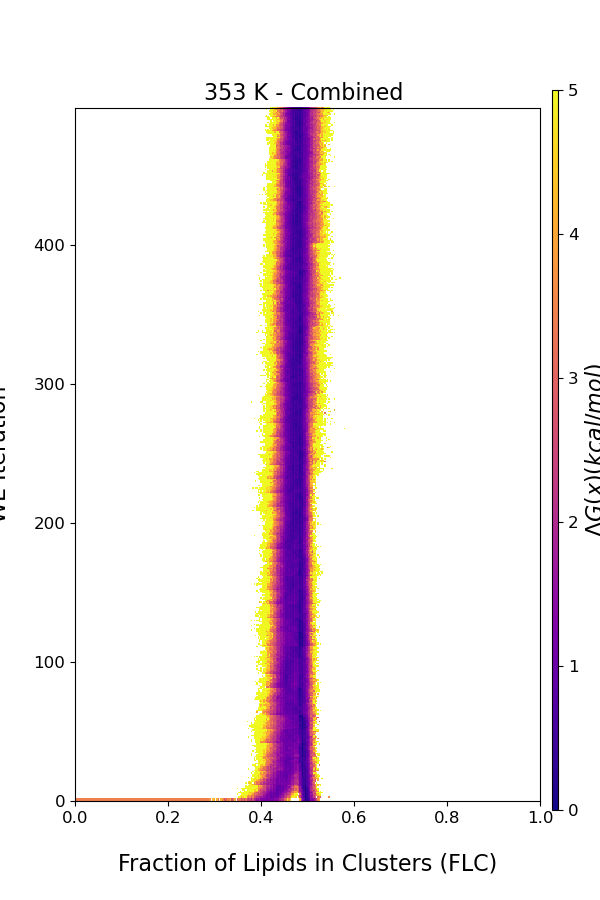
\includegraphics[width=0.8\linewidth]{all_plots/ClusterLipids2Total/DPPC_DAPC_CHOL/353K/Evolution_DAPC_MULTI__353_ClusterLipids2Total.png}
\caption{Evolution of Free Energy Landscape of \textbf{DAPC} system for combined replicas at 353K using w\_multi\_tool.}
\label{fig:view}

\end{figure}

% --------- %

\begin{figure}[hbt!]
\centering
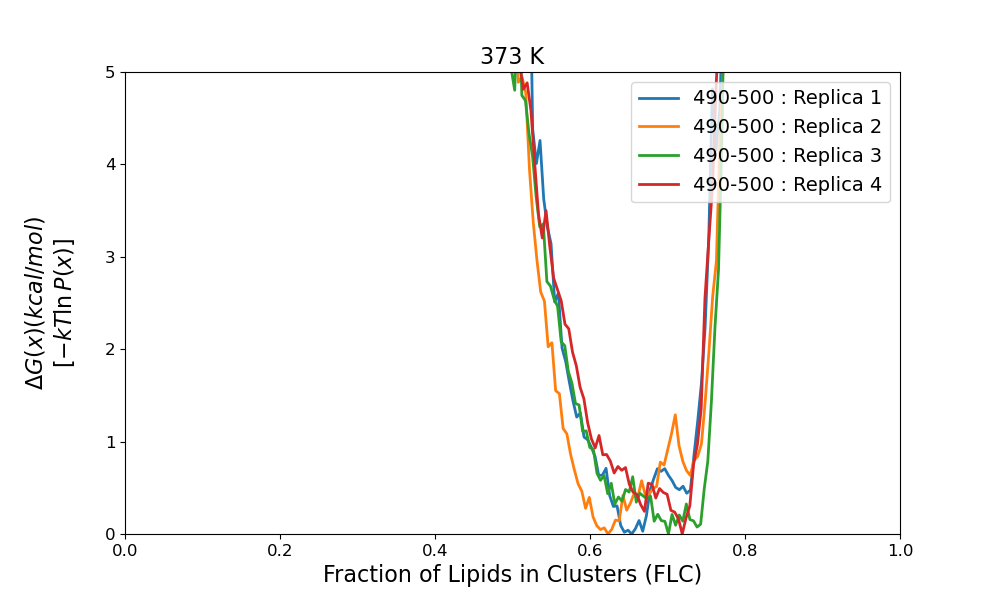
\includegraphics[width=1.1\linewidth]{all_plots/ClusterLipids2Total/DPPC_DAPC_CHOL/373K/Average_DAPC_373_ClusterLipids2Total.png}
\caption{Free Energy Landscape of \textbf{DAPC} system for different replicas at 373K. All the FES are calculated by averaging over the iteration window 490 - 500.}
\label{fig:view}

\end{figure}

\begin{figure}[hbt!]
\centering
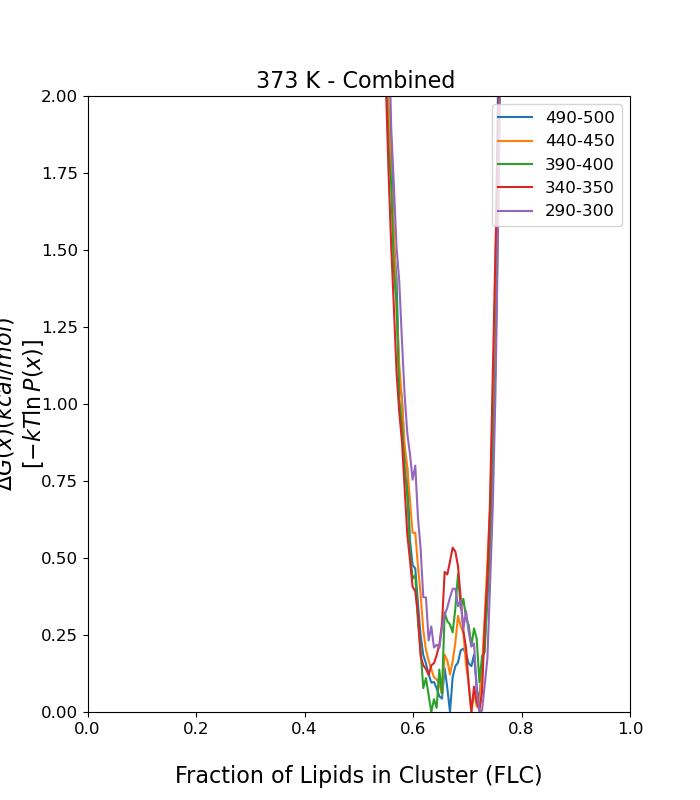
\includegraphics[width=0.6\linewidth]{all_plots/ClusterLipids2Total/DPPC_DAPC_CHOL/373K/Convergence_DAPC_MULTI__373_ClusterLipids2Total.png}
\caption{Convergence of Free Energy Landscape of \textbf{DAPC} system for combined replicas at 373K. All the FES are calculated by averaging over the iteration window 490 - 500.}
\label{fig:view}

\end{figure}

\begin{figure}[hbt!]
\centering
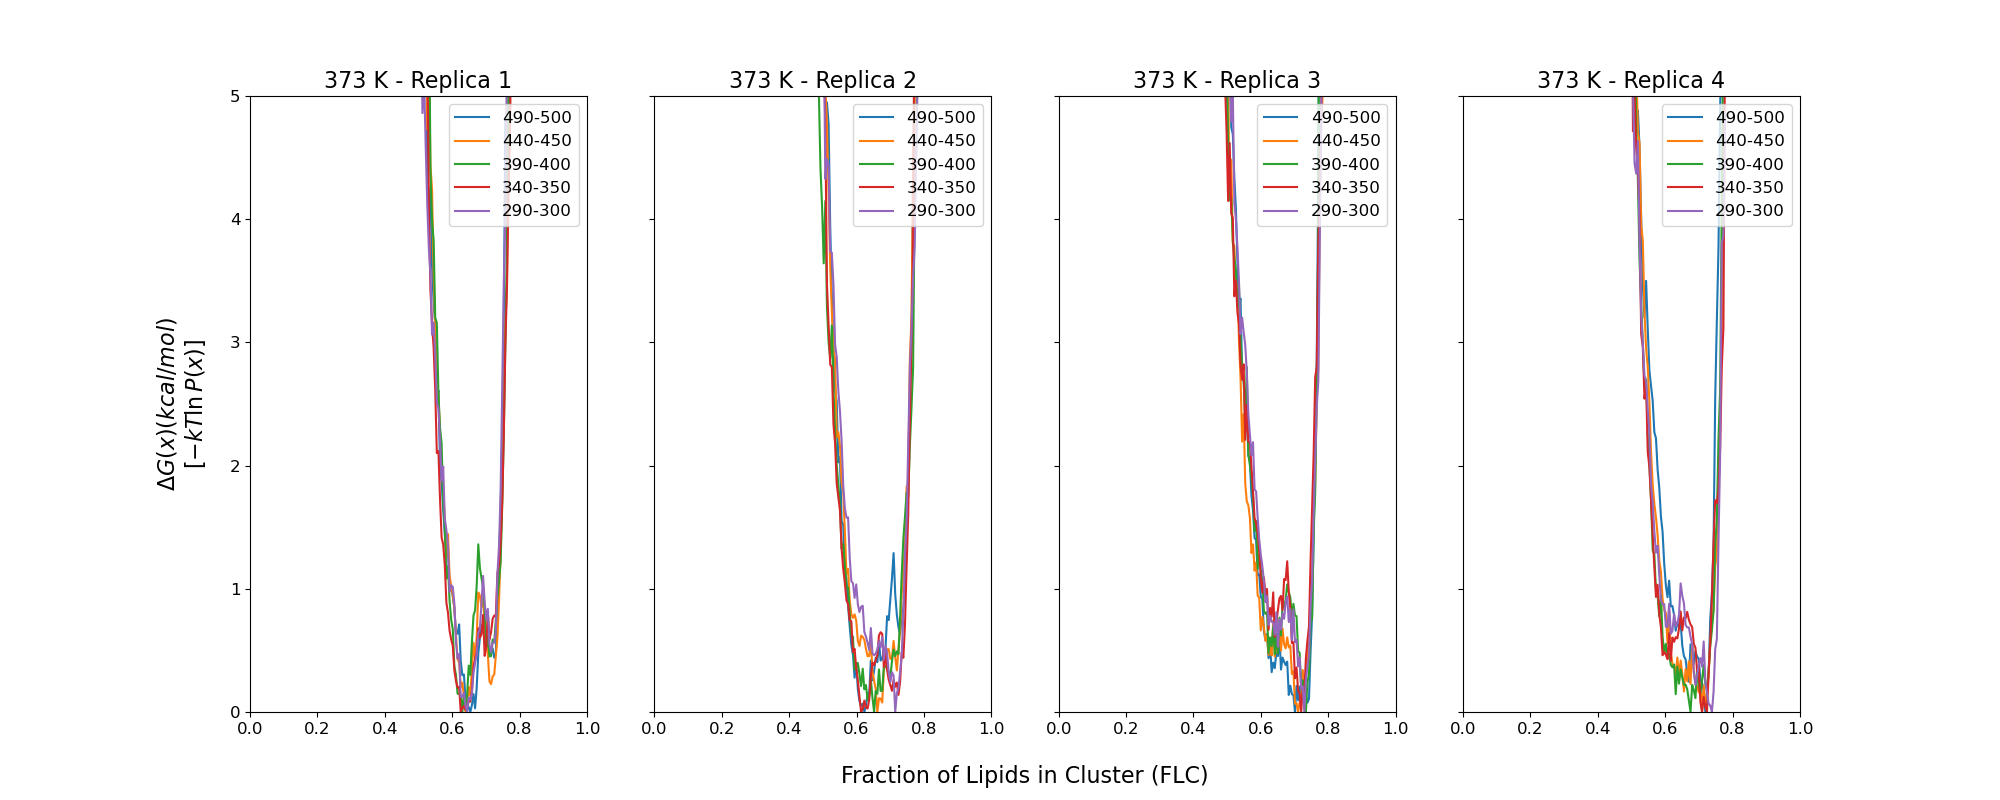
\includegraphics[width=1.1\linewidth]{all_plots/ClusterLipids2Total/DPPC_DAPC_CHOL/373K/Convergence_DAPC_373_ClusterLipids2Total.png}
\caption{Convergence of Free Energy Landscape of \textbf{DAPC} system for different replicas at 373K. All the FES are calculated by averaging over the iteration window 490 - 500.}
\label{fig:view}

\end{figure}

\begin{figure}[hbt!]
\centering
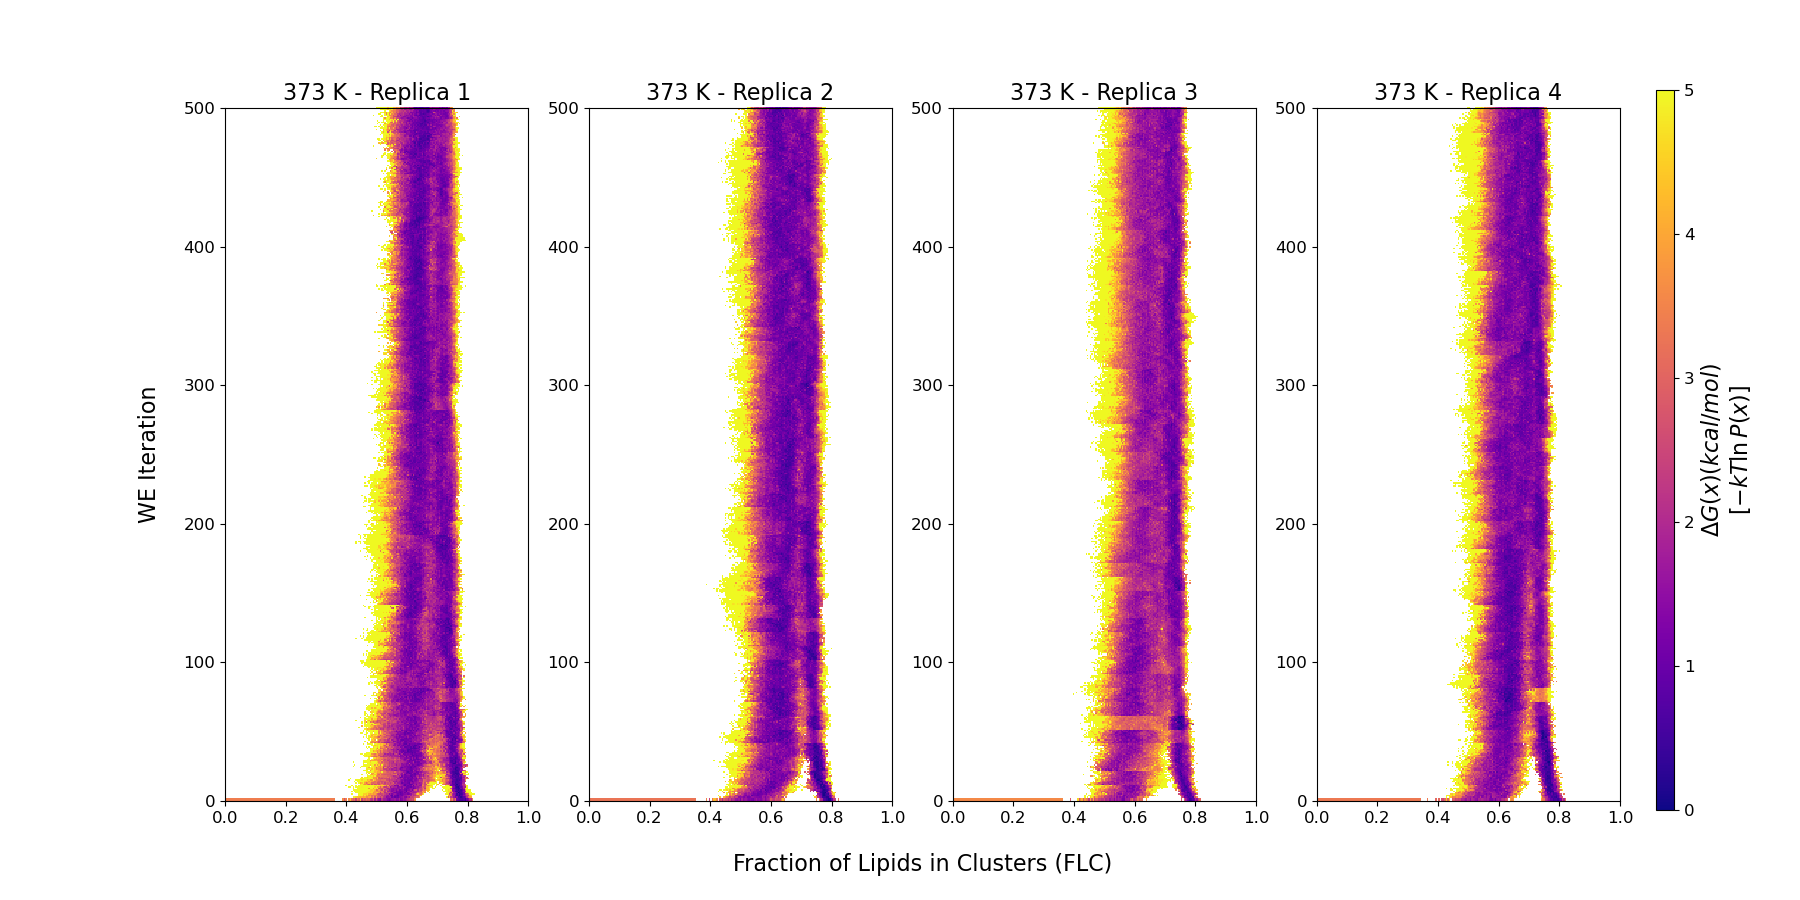
\includegraphics[width=1.1\linewidth]{all_plots/ClusterLipids2Total/DPPC_DAPC_CHOL/373K/Evolution_DAPC_373_ClusterLipids2Total.png}
\caption{Evolution of Free Energy Landscape of \textbf{DAPC} system for different replicas at 373K.}
\label{fig:view}

\end{figure}

\begin{figure}[hbt!]
\centering
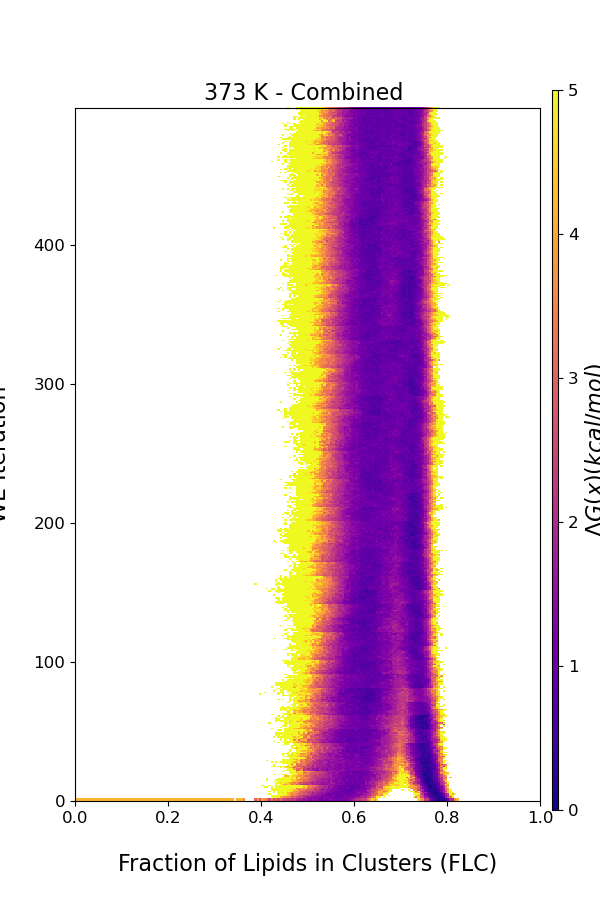
\includegraphics[width=0.8\linewidth]{all_plots/ClusterLipids2Total/DPPC_DAPC_CHOL/373K/Evolution_DAPC_MULTI__373_ClusterLipids2Total.png}
\caption{Evolution of Free Energy Landscape of \textbf{DAPC} system for combined replicas at 373K using w\_multi\_tool.}
\label{fig:view}

\end{figure}

%---------------------%

\begin{figure}[hbt!]
\centering
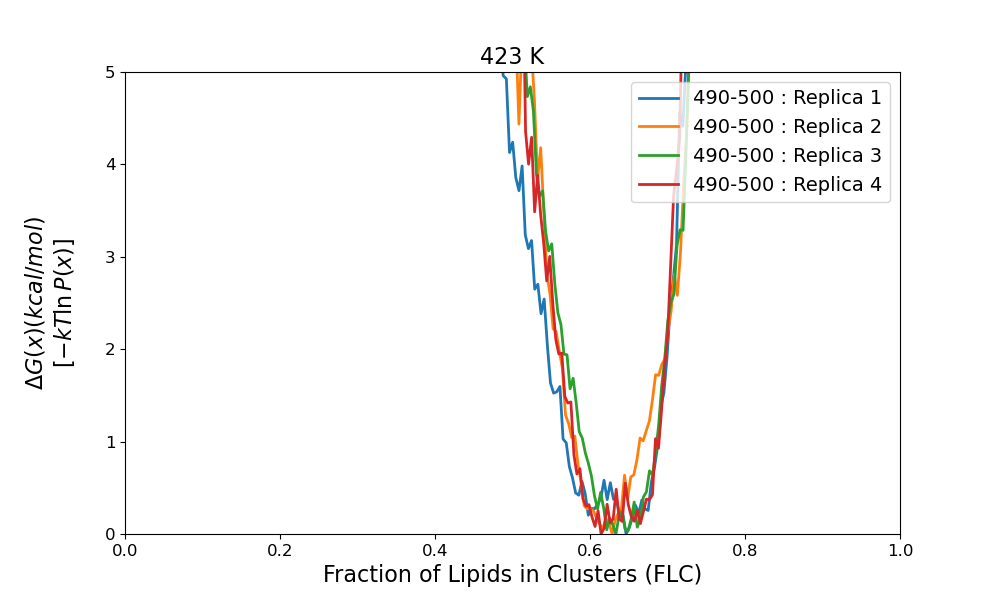
\includegraphics[width=1.1\linewidth]{all_plots/ClusterLipids2Total/DPPC_DAPC_CHOL/423K/Average_DAPC_423_ClusterLipids2Total.png}
\caption{Free Energy Landscape of \textbf{DAPC} system for different replicas at 423K. All the FES are calculated by averaging over the iteration window 490 - 500.}
\label{fig:view}

\end{figure}

\begin{figure}[hbt!]
\centering
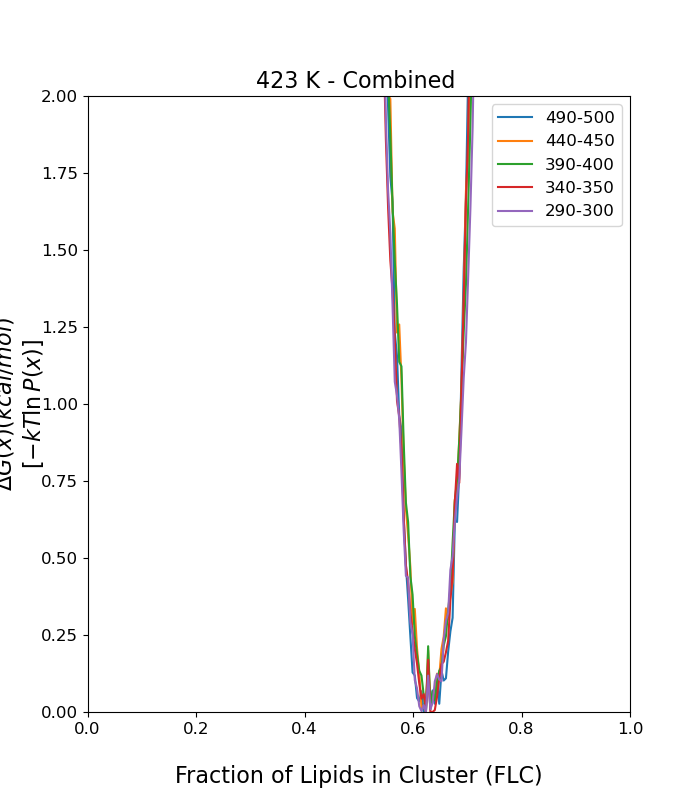
\includegraphics[width=0.6\linewidth]{all_plots/ClusterLipids2Total/DPPC_DAPC_CHOL/423K/Convergence_DAPC_MULTI__423_ClusterLipids2Total.png}
\caption{Convergence of Free Energy Landscape of \textbf{DAPC} system for combined replicas at 423K. All the FES are calculated by averaging over the iteration window 490 - 500.}
\label{fig:view}

\end{figure}

\begin{figure}[hbt!]
\centering
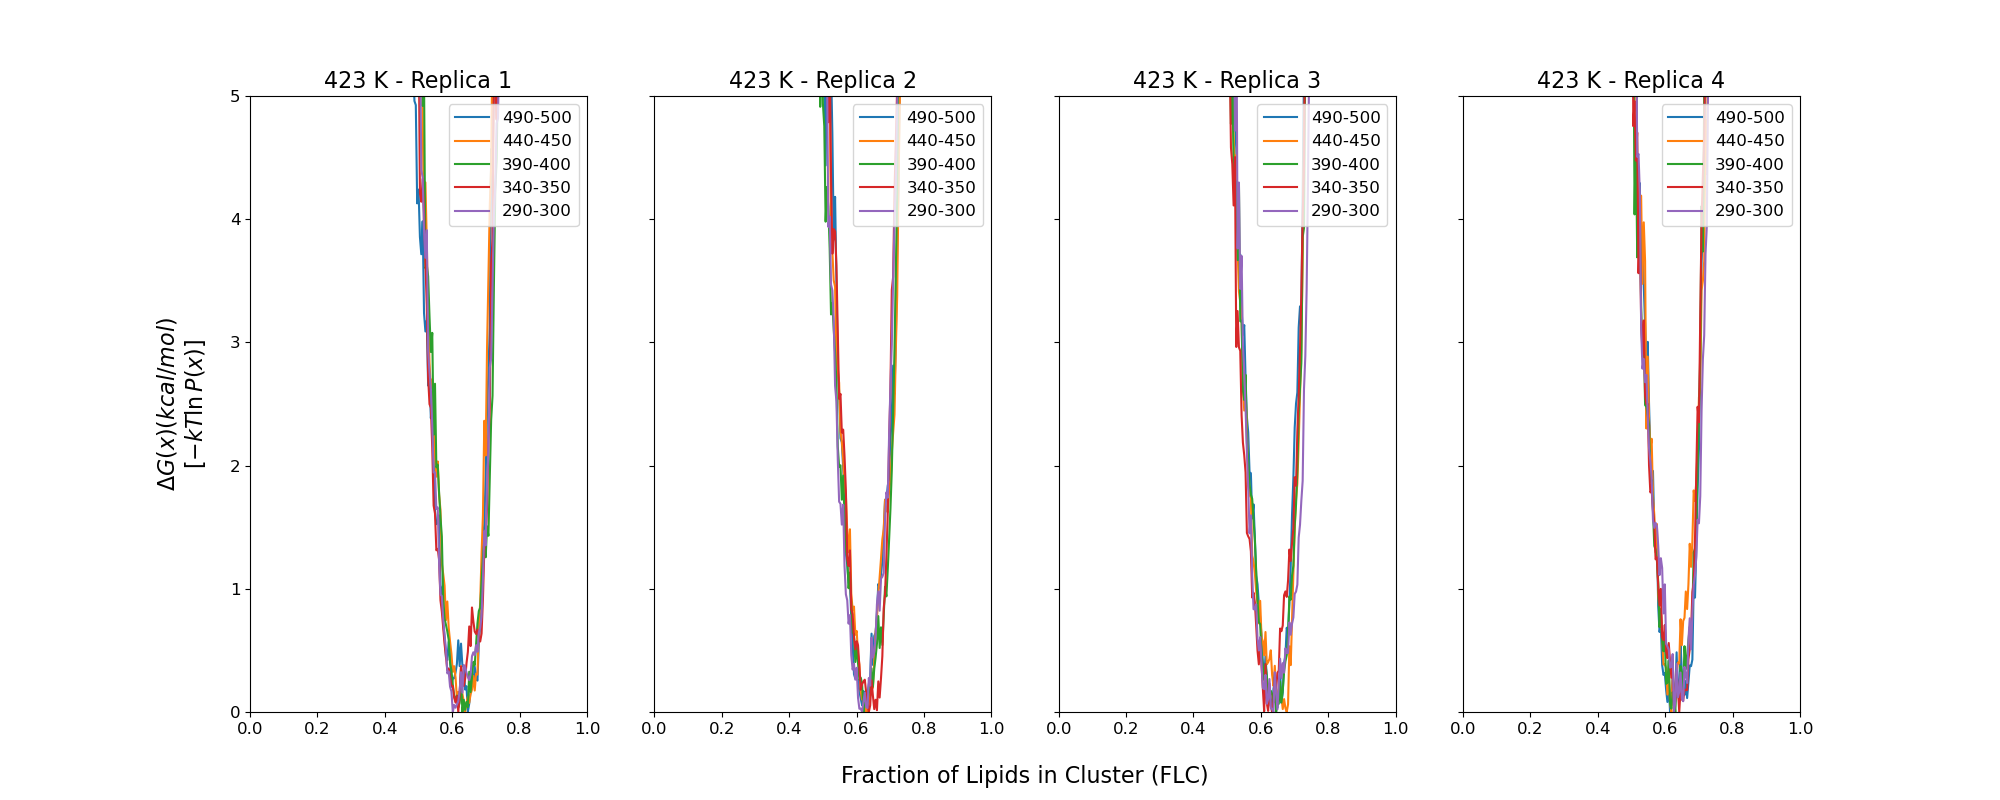
\includegraphics[width=1.1\linewidth]{all_plots/ClusterLipids2Total/DPPC_DAPC_CHOL/423K/Convergence_DAPC_423_ClusterLipids2Total.png}
\caption{Convergence of Free Energy Landscape of \textbf{DAPC} system for different replicas at 423K. All the FES are calculated by averaging over the iteration window 490 - 500.}
\label{fig:view}

\end{figure}

\begin{figure}[hbt!]
\centering
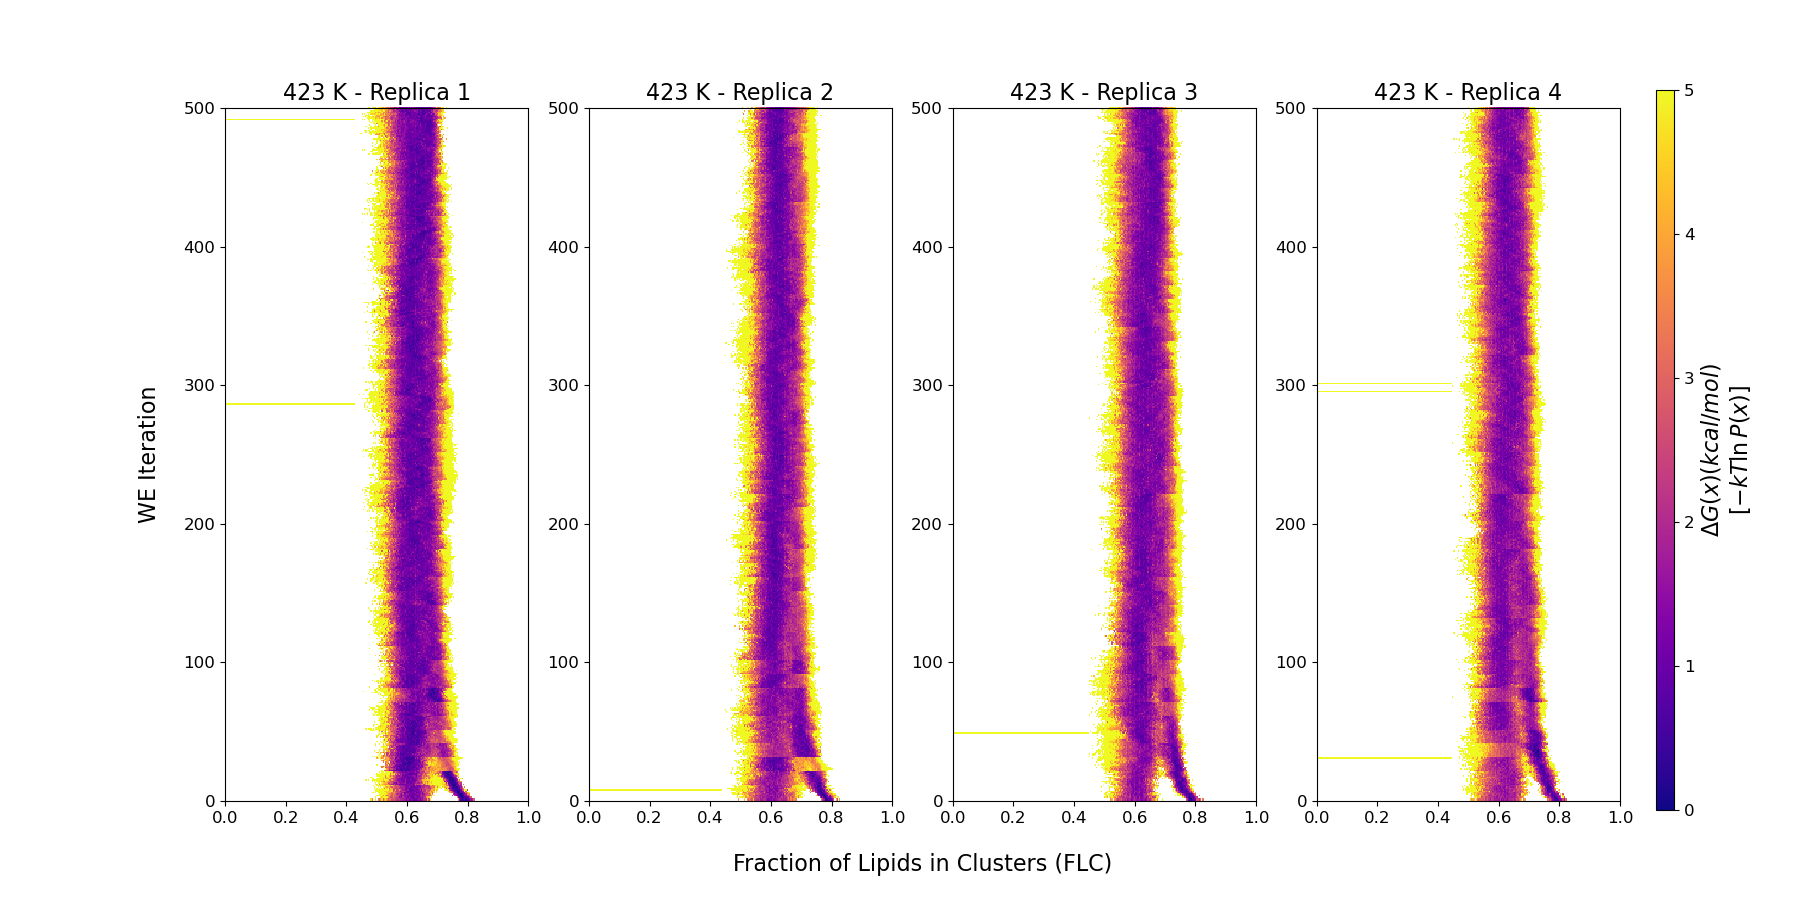
\includegraphics[width=1.1\linewidth]{all_plots/ClusterLipids2Total/DPPC_DAPC_CHOL/423K/Evolution_DAPC_423_ClusterLipids2Total.png}
\caption{Evolution of Free Energy Landscape of \textbf{DAPC} system for different replicas at 423K.}
\label{fig:view}

\end{figure}

\begin{figure}[hbt!]
\centering
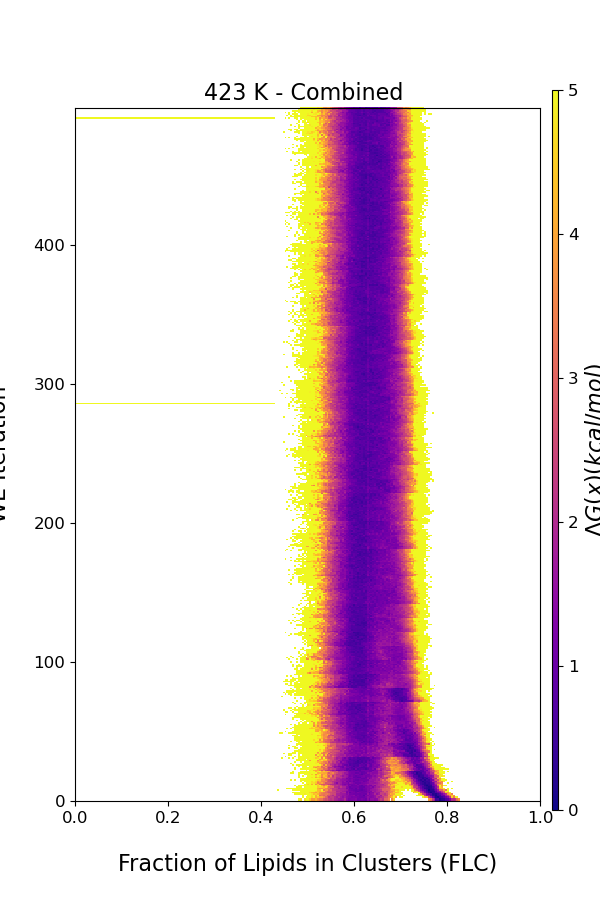
\includegraphics[width=0.8\linewidth]{all_plots/ClusterLipids2Total/DPPC_DAPC_CHOL/423K/Evolution_DAPC_MULTI__423_ClusterLipids2Total.png}
\caption{Evolution of Free Energy Landscape of \textbf{DAPC} system for combined replicas at 423K using w\_multi\_tool.}
\label{fig:view}

\end{figure}

%---------------------%

% ########################################### %

%---------------------%

\begin{figure}[hbt!]
\centering
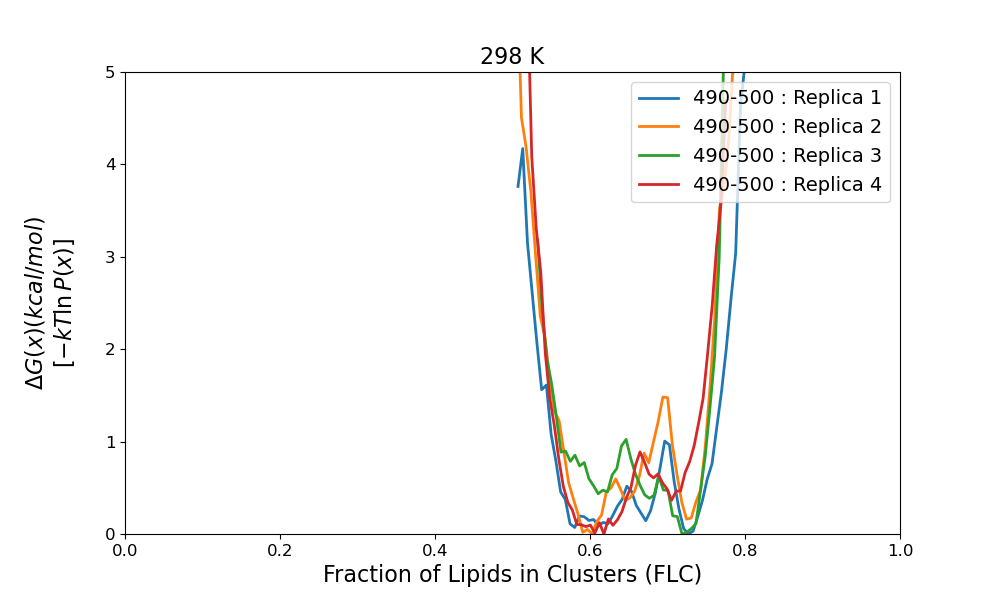
\includegraphics[width=1.1\linewidth]{all_plots/ClusterLipids2Total/DPPC_DIPC_CHOL/298K/Average_DIPC_298_ClusterLipids2Total.png}
\caption{Free Energy Landscape of \textbf{DIPC} system for different replicas at 298K. All the FES are calculated by averaging over the iteration window 490 - 500.}
\label{fig:view}

\end{figure}

\begin{figure}[hbt!]
\centering
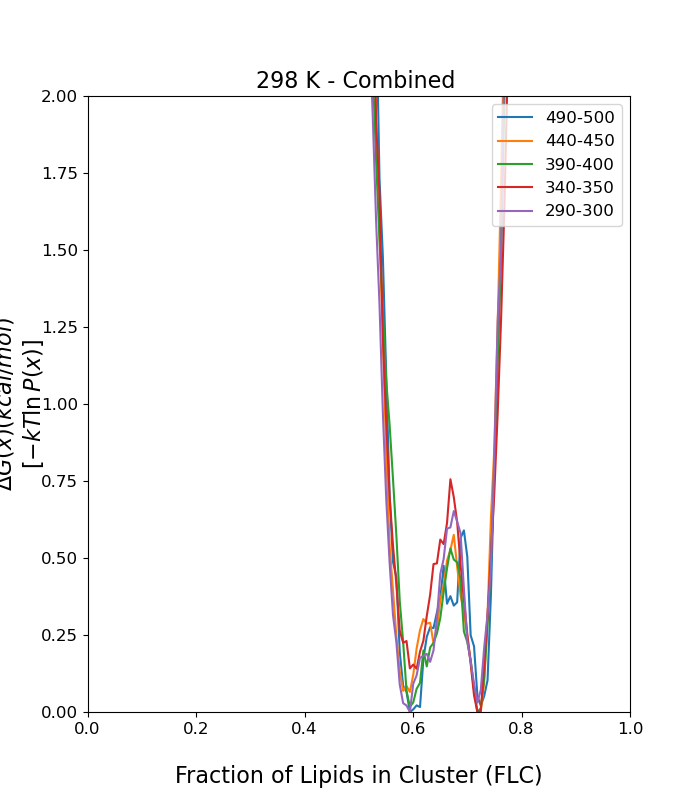
\includegraphics[width=0.6\linewidth]{all_plots/ClusterLipids2Total/DPPC_DIPC_CHOL/298K/Convergence_DIPC_MULTI__298_ClusterLipids2Total.png}
\caption{Convergence of Free Energy Landscape of \textbf{DIPC} system for combined replicas at 298K. All the FES are calculated by averaging over the iteration window 490 - 500.}
\label{fig:view}

\end{figure}

\begin{figure}[hbt!]
\centering
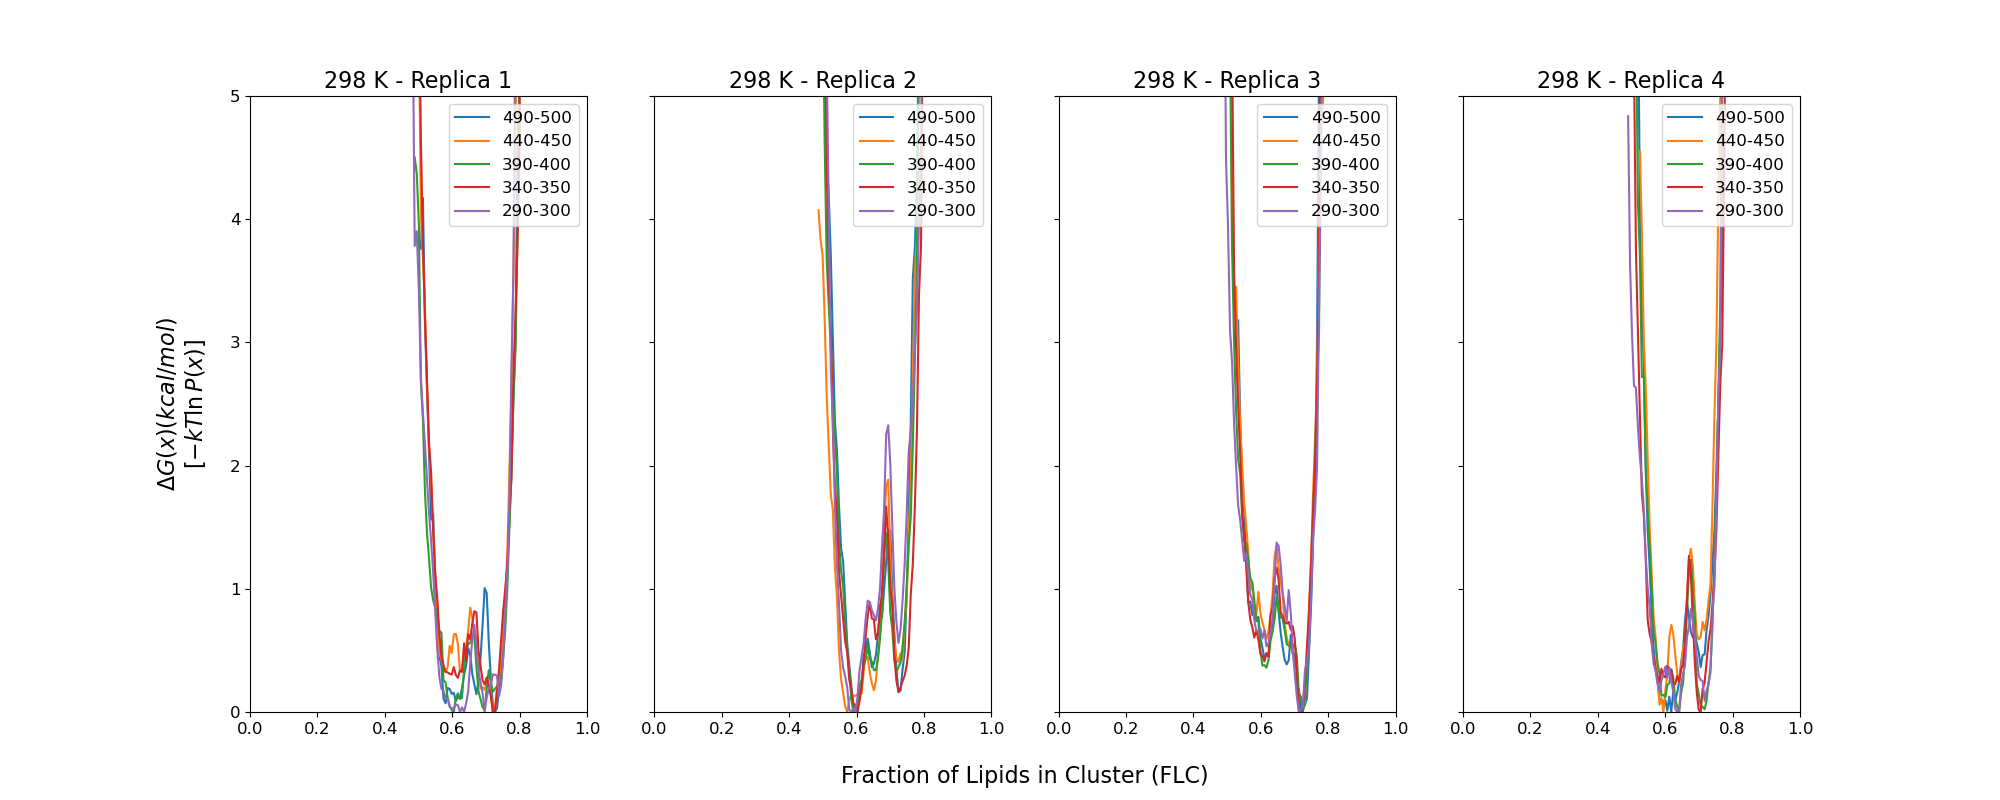
\includegraphics[width=1.1\linewidth]{all_plots/ClusterLipids2Total/DPPC_DIPC_CHOL/298K/Convergence_DIPC_298_ClusterLipids2Total.png}
\caption{Convergence of Free Energy Landscape of \textbf{DIPC} system for different replicas at 298K. All the FES are calculated by averaging over the iteration window 490 - 500.}
\label{fig:view}

\end{figure}

\begin{figure}[hbt!]
\centering
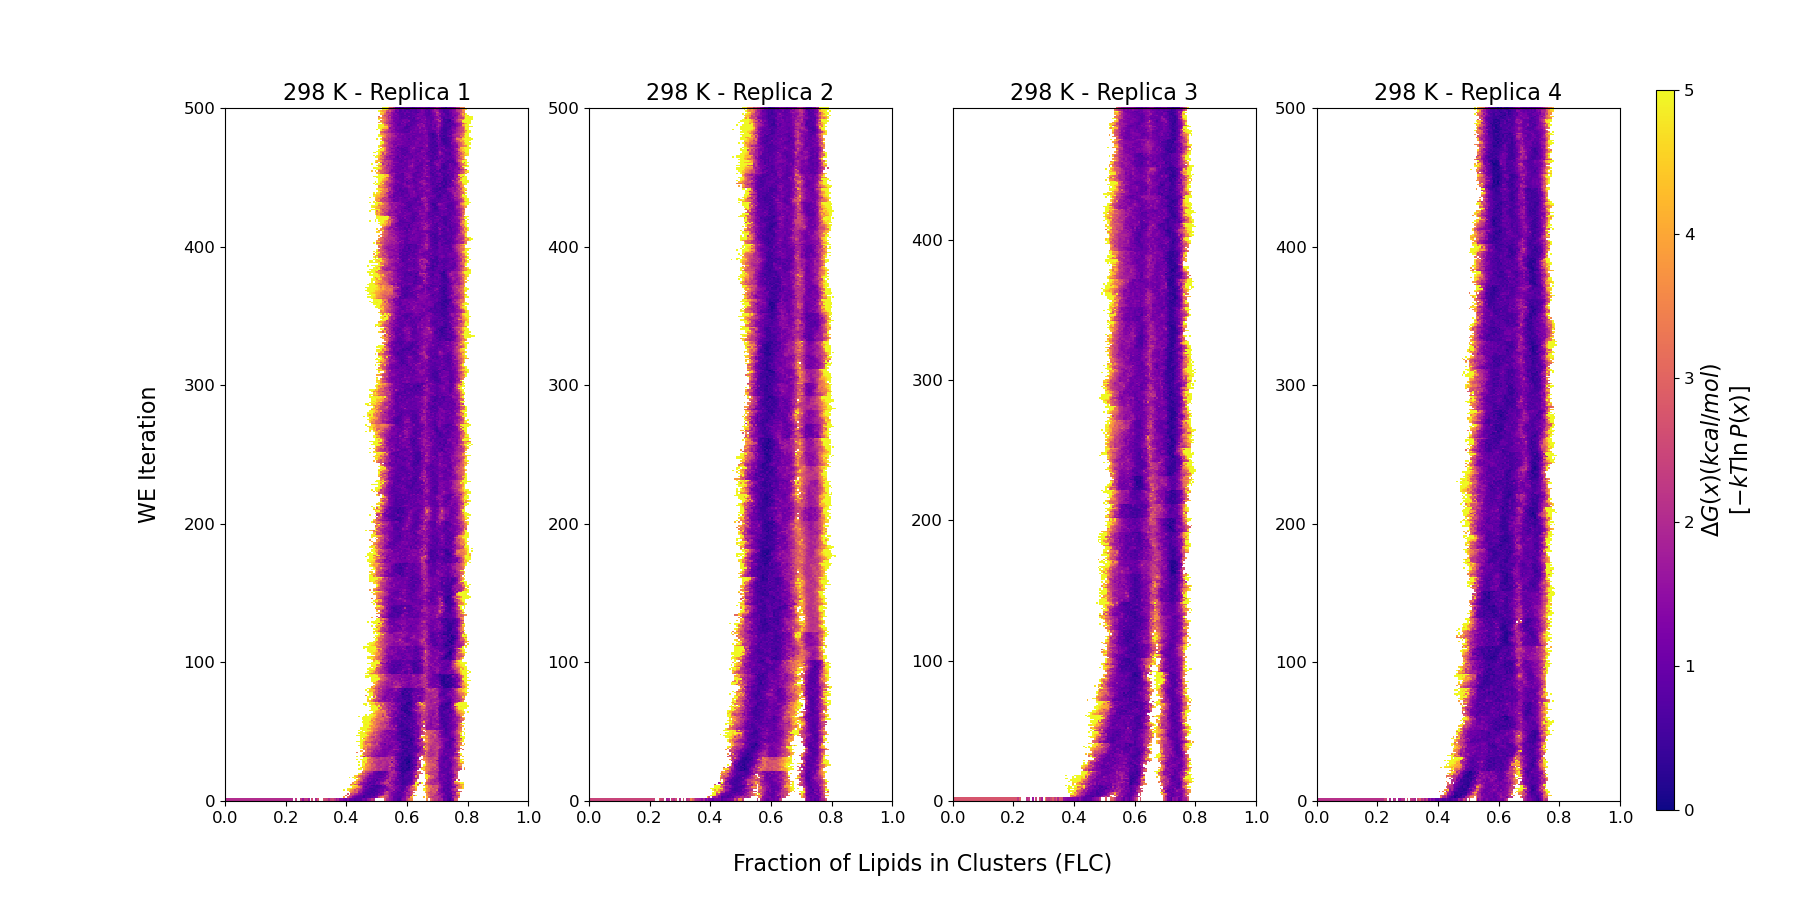
\includegraphics[width=1.1\linewidth]{all_plots/ClusterLipids2Total/DPPC_DIPC_CHOL/298K/Evolution_DIPC_298_ClusterLipids2Total.png}
\caption{Evolution of Free Energy Landscape of \textbf{DIPC} system for different replicas at 298K.}
\label{fig:view}

\end{figure}

\begin{figure}[hbt!]
\centering
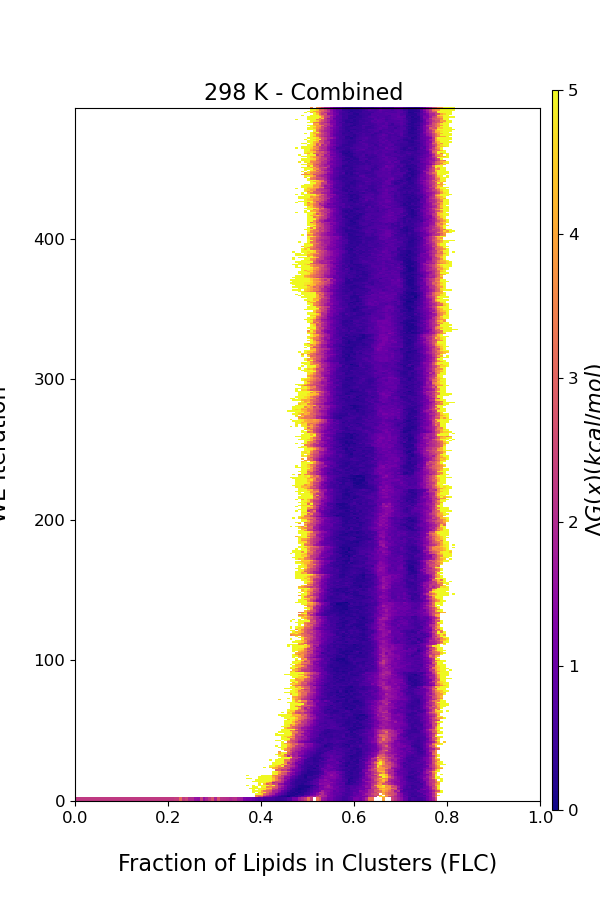
\includegraphics[width=0.8\linewidth]{all_plots/ClusterLipids2Total/DPPC_DIPC_CHOL/298K/Evolution_DIPC_MULTI__298_ClusterLipids2Total.png}
\caption{Evolution of Free Energy Landscape of \textbf{DIPC} system for combined replicas at 298K using w\_multi\_tool.}
\label{fig:view}

\end{figure}

%---------------------%

\begin{figure}[hbt!]
\centering
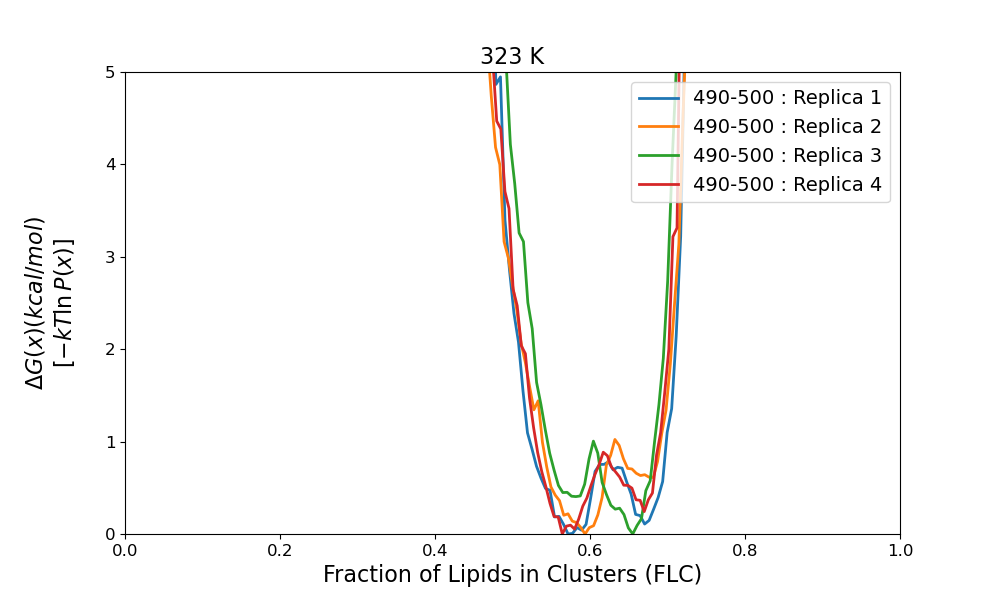
\includegraphics[width=1.1\linewidth]{all_plots/ClusterLipids2Total/DPPC_DIPC_CHOL/323K/Average_DIPC_323_ClusterLipids2Total.png}
\caption{Free Energy Landscape of \textbf{DIPC} system for different replicas at 323K. All the FES are calculated by averaging over the iteration window 490 - 500.}
\label{fig:view}

\end{figure}

\begin{figure}[hbt!]
\centering
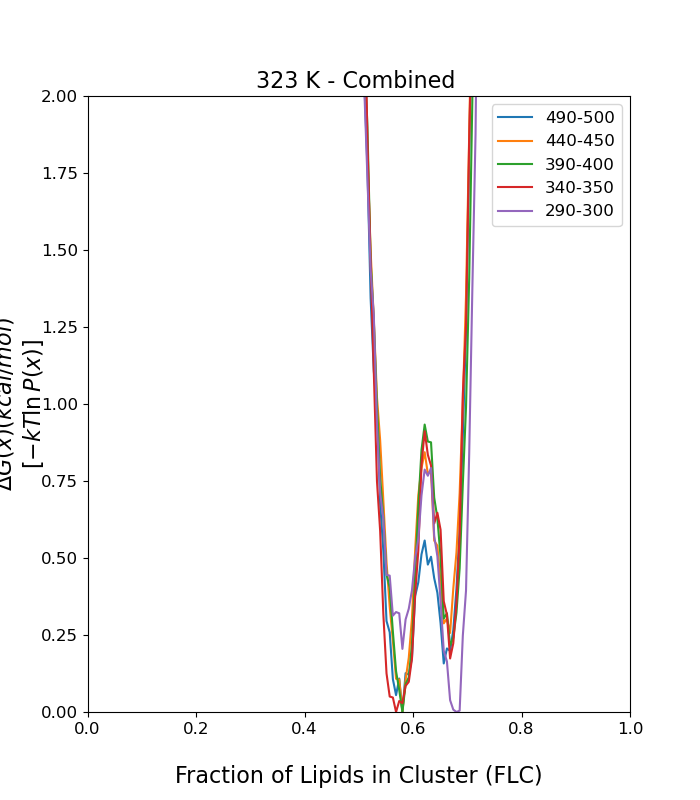
\includegraphics[width=0.6\linewidth]{all_plots/ClusterLipids2Total/DPPC_DIPC_CHOL/323K/Convergence_DIPC_MULTI__323_ClusterLipids2Total.png}
\caption{Convergence of Free Energy Landscape of \textbf{DIPC} system for combined replicas at 323K. All the FES are calculated by averaging over the iteration window 490 - 500.}
\label{fig:view}

\end{figure}

\begin{figure}[hbt!]
\centering
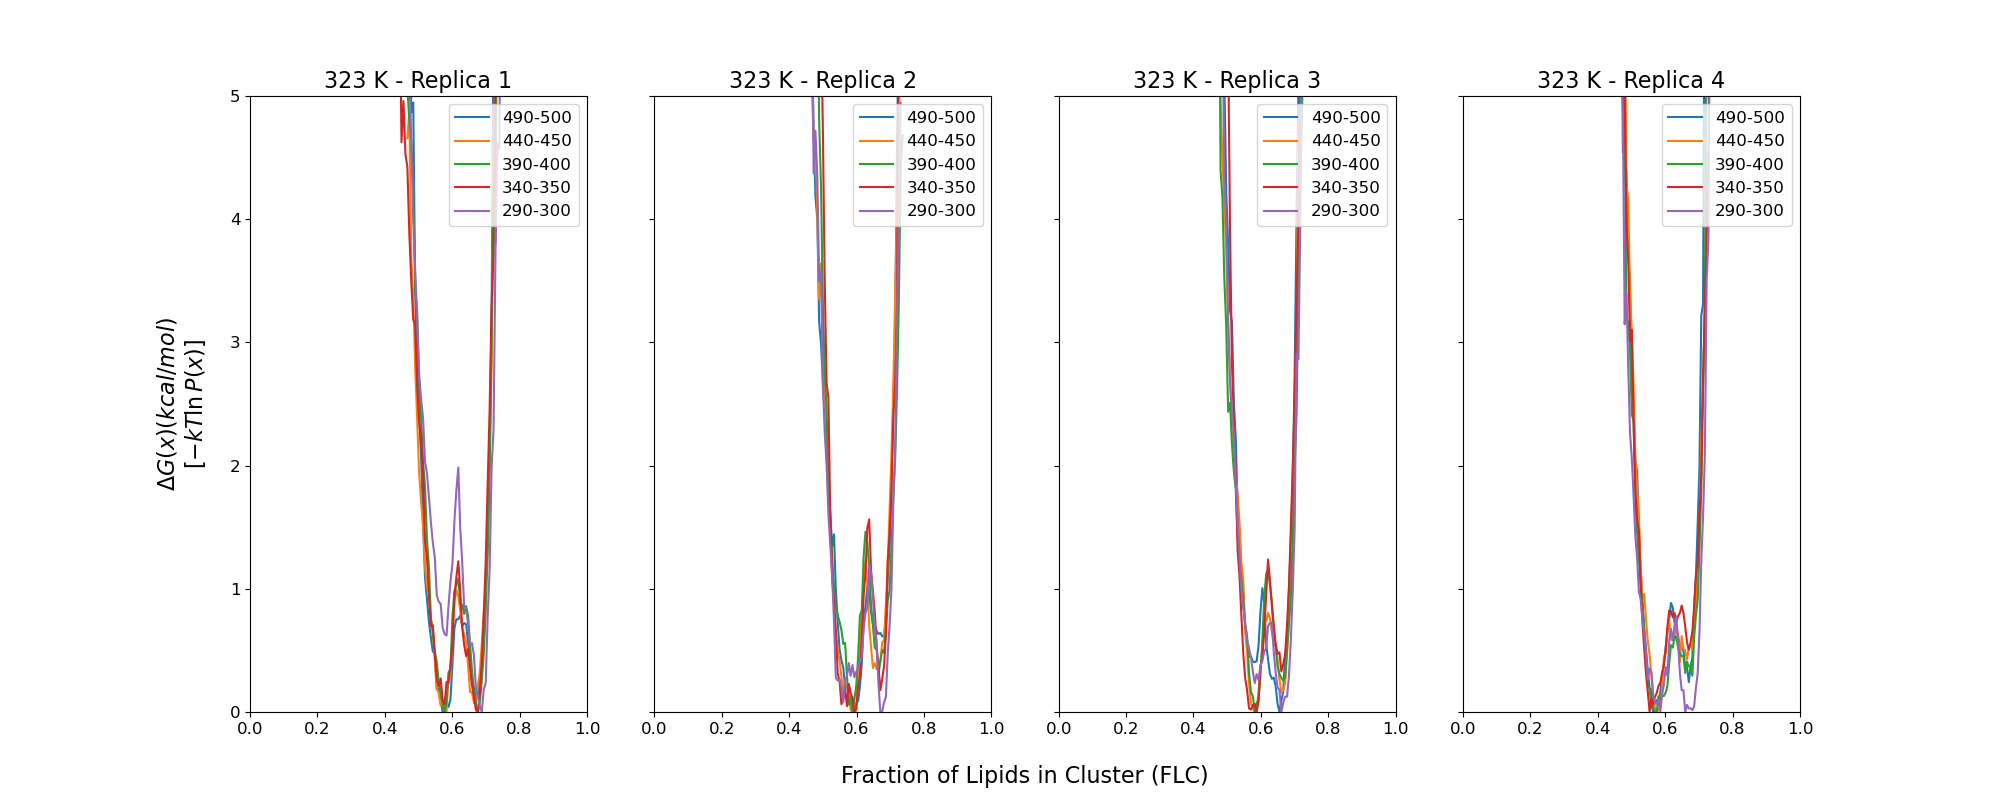
\includegraphics[width=1.1\linewidth]{all_plots/ClusterLipids2Total/DPPC_DIPC_CHOL/323K/Convergence_DIPC_323_ClusterLipids2Total.png}
\caption{Convergence of Free Energy Landscape of \textbf{DIPC} system for different replicas at 323K. All the FES are calculated by averaging over the iteration window 490 - 500.}
\label{fig:view}

\end{figure}

\begin{figure}[hbt!]
\centering
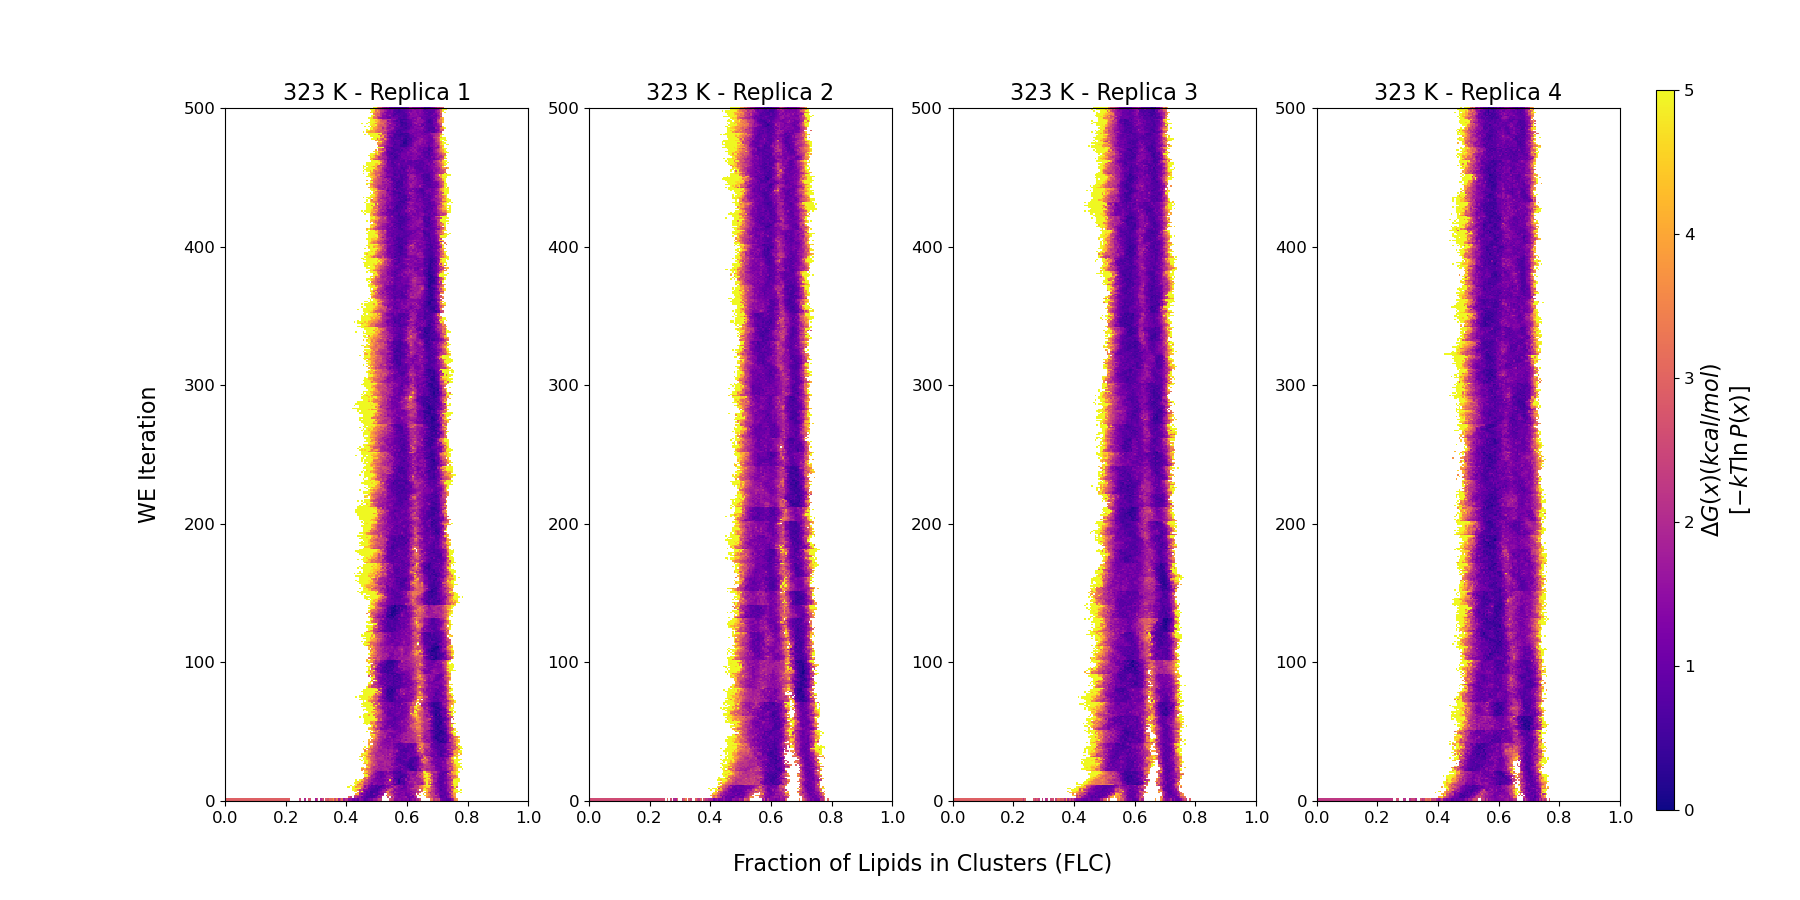
\includegraphics[width=1.1\linewidth]{all_plots/ClusterLipids2Total/DPPC_DIPC_CHOL/323K/Evolution_DIPC_323_ClusterLipids2Total.png}
\caption{Evolution of Free Energy Landscape of \textbf{DIPC} system for different replicas at 323K.}
\label{fig:view}

\end{figure}

\begin{figure}[hbt!]
\centering
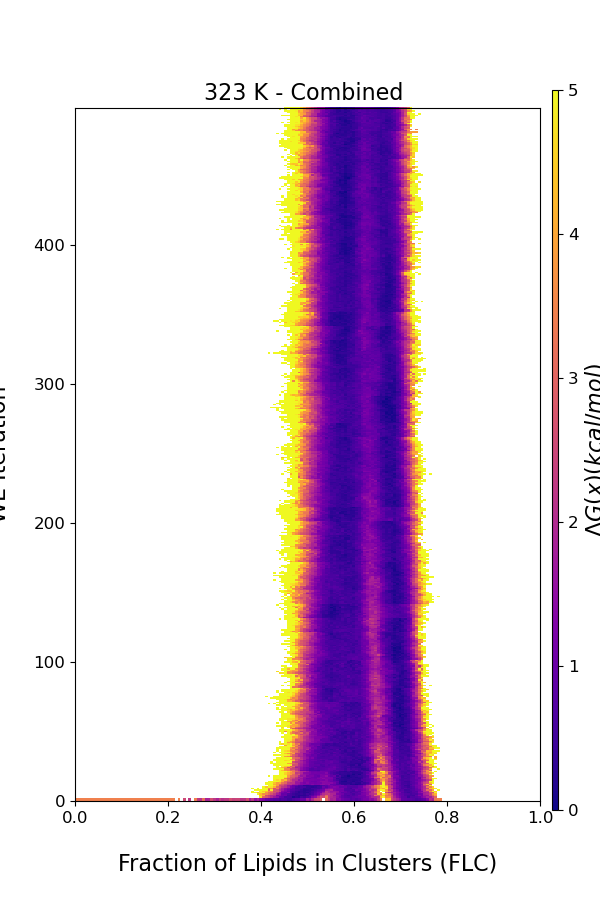
\includegraphics[width=0.8\linewidth]{all_plots/ClusterLipids2Total/DPPC_DIPC_CHOL/323K/Evolution_DIPC_MULTI__323_ClusterLipids2Total.png}
\caption{Evolution of Free Energy Landscape of \textbf{DIPC} system for combined replicas at 323K using w\_multi\_tool.}
\label{fig:view}

\end{figure}

%---------------------%

\begin{figure}[hbt!]
\centering
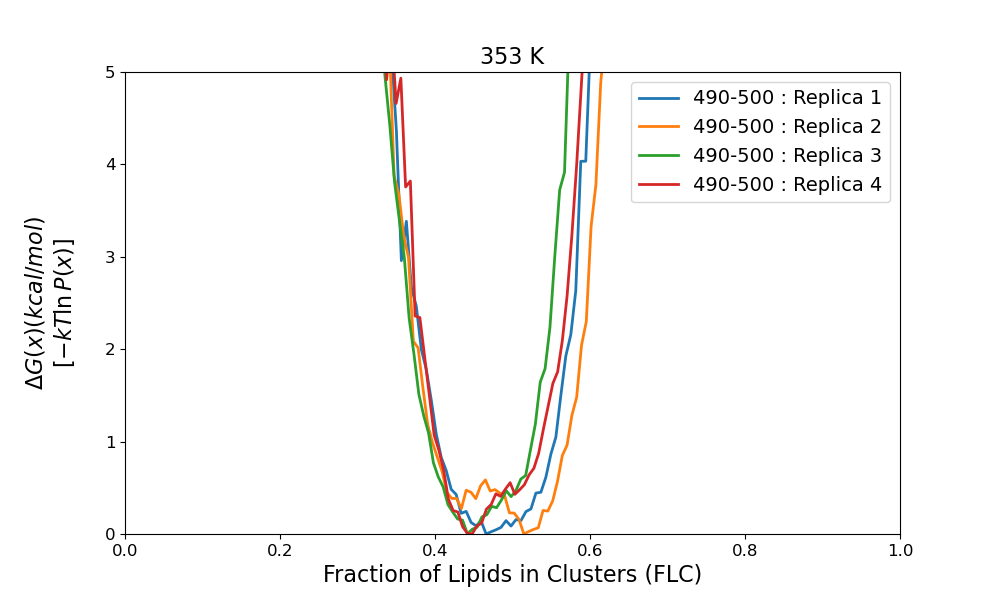
\includegraphics[width=1.1\linewidth]{all_plots/ClusterLipids2Total/DPPC_DIPC_CHOL/353K/Average_DIPC_353_ClusterLipids2Total.png}
\caption{Free Energy Landscape of \textbf{DIPC} system for different replicas at 353K. All the FES are calculated by averaging over the iteration window 490 - 500.}
\label{fig:view}

\end{figure}

\begin{figure}[hbt!]
\centering
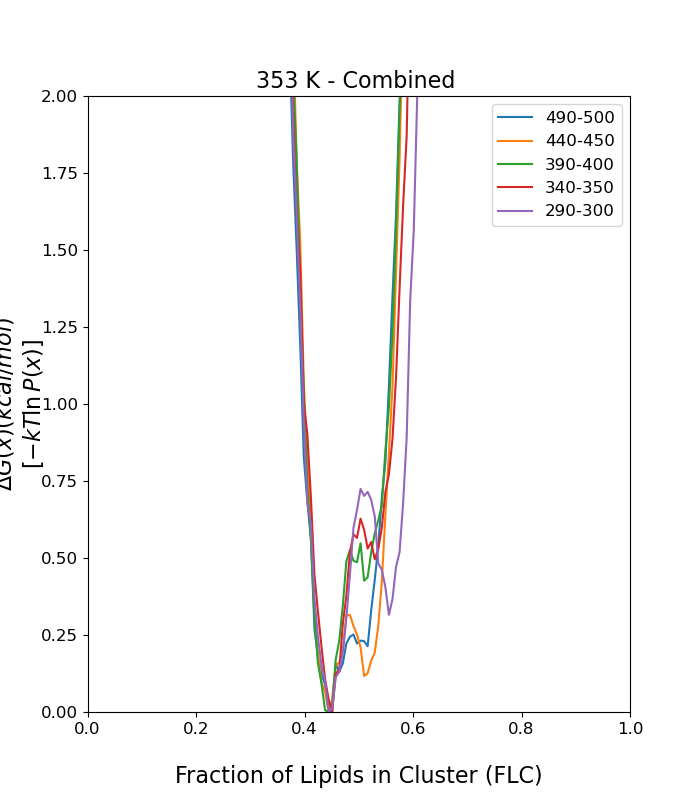
\includegraphics[width=0.6\linewidth]{all_plots/ClusterLipids2Total/DPPC_DIPC_CHOL/353K/Convergence_DIPC_MULTI__353_ClusterLipids2Total.png}
\caption{Convergence of Free Energy Landscape of \textbf{DIPC} system for combined replicas at 353K. All the FES are calculated by averaging over the iteration window 490 - 500.}
\label{fig:view}

\end{figure}

\begin{figure}[hbt!]
\centering
\includegraphics[width=1.1\linewidth]{all_plots/ClusterLipids2Total/DPPC_DIPC_CHOL/353K/Convergence_DIPC_353_ClusterLipids2Total.png}
\caption{Convergence of Free Energy Landscape of \textbf{DIPC} system for different replicas at 353K. All the FES are calculated by averaging over the iteration window 490 - 500.}
\label{fig:view}

\end{figure}

\begin{figure}[hbt!]
\centering
\includegraphics[width=1.1\linewidth]{all_plots/ClusterLipids2Total/DPPC_DIPC_CHOL/353K/Evolution_DIPC_353_ClusterLipids2Total.png}
\caption{Evolution of Free Energy Landscape of \textbf{DIPC} system for different replicas at 353K.}
\label{fig:view}

\end{figure}

\clearpage

\begin{figure}[hbt!]
\centering
\includegraphics[width=0.8\linewidth]{all_plots/ClusterLipids2Total/DPPC_DIPC_CHOL/353K/Evolution_DIPC_MULTI__353_ClusterLipids2Total.png}
\caption{Evolution of Free Energy Landscape of \textbf{DIPC} system for combined replicas at 353K using w\_multi\_tool.}
\label{fig:view}

\end{figure}

%---------------------%

\begin{figure}[hbt!]
\centering
\includegraphics[width=1.1\linewidth]{all_plots/ClusterLipids2Total/DPPC_DIPC_CHOL/423K/Average_DIPC_423_ClusterLipids2Total.png}
\caption{Free Energy Landscape of \textbf{DIPC} system for different replicas at 423K. All the FES are calculated by averaging over the iteration window 490 - 500.}
\label{fig:view}

\end{figure}

\begin{figure}[hbt!]
\centering
\includegraphics[width=0.6\linewidth]{all_plots/ClusterLipids2Total/DPPC_DIPC_CHOL/423K/Convergence_DIPC_MULTI__423_ClusterLipids2Total.png}
\caption{Convergence of Free Energy Landscape of \textbf{DIPC} system for combined replicas at 423K. All the FES are calculated by averaging over the iteration window 490 - 500.}
\label{fig:view}

\end{figure}

\begin{figure}[hbt!]
\centering
\includegraphics[width=1.1\linewidth]{all_plots/ClusterLipids2Total/DPPC_DIPC_CHOL/423K/Convergence_DIPC_423_ClusterLipids2Total.png}
\caption{Convergence of Free Energy Landscape of \textbf{DIPC} system for different replicas at 423K. All the FES are calculated by averaging over the iteration window 490 - 500.}
\label{fig:view}

\end{figure}

\begin{figure}[hbt!]
\centering
\includegraphics[width=1.1\linewidth]{all_plots/ClusterLipids2Total/DPPC_DIPC_CHOL/423K/Evolution_DIPC_423_ClusterLipids2Total.png}
\caption{Evolution of Free Energy Landscape of \textbf{DIPC} system for different replicas at 423K.}
\label{fig:view}

\end{figure}

\begin{figure}[hbt!]
\centering
\includegraphics[width=0.8\linewidth]{all_plots/ClusterLipids2Total/DPPC_DIPC_CHOL/423K/Evolution_DIPC_MULTI__423_ClusterLipids2Total.png}
\caption{Evolution of Free Energy Landscape of \textbf{DIPC} system for combined replicas at 423K using w\_multi\_tool.}
\label{fig:view}

\end{figure}

% ------------------ %

% ###################################### %

%---------------------%

\begin{figure}[hbt!]
\centering
\includegraphics[width=1.1\linewidth]{all_plots/ClusterLipids2Total/DPPC_POPC_CHOL/298K/Average_POPC_298_ClusterLipids2Total.png}
\caption{Free Energy Landscape of \textbf{POPC} system for different replicas at 298K. All the FES are calculated by averaging over the iteration window 490 - 500.}
\label{fig:view}

\end{figure}

\begin{figure}[hbt!]
\centering
\includegraphics[width=0.6\linewidth]{all_plots/ClusterLipids2Total/DPPC_POPC_CHOL/298K/Convergence_POPC_MULTI__298_ClusterLipids2Total.png}
\caption{Convergence of Free Energy Landscape of \textbf{POPC} system for combined replicas at 298K. All the FES are calculated by averaging over the iteration window 490 - 500.}
\label{fig:view}

\end{figure}

\begin{figure}[hbt!]
\centering
\includegraphics[width=1.1\linewidth]{all_plots/ClusterLipids2Total/DPPC_POPC_CHOL/298K/Convergence_POPC_298_ClusterLipids2Total.png}
\caption{Convergence of Free Energy Landscape of \textbf{POPC} system for different replicas at 298K. All the FES are calculated by averaging over the iteration window 490 - 500.}
\label{fig:view}

\end{figure}

\begin{figure}[hbt!]
\centering
\includegraphics[width=1.1\linewidth]{all_plots/ClusterLipids2Total/DPPC_POPC_CHOL/298K/Evolution_POPC_298_ClusterLipids2Total.png}
\caption{Evolution of Free Energy Landscape of \textbf{POPC} system for different replica at 298K.}
\label{fig:view}

\end{figure}

\begin{figure}[hbt!]
\centering
\includegraphics[width=0.8\linewidth]{all_plots/ClusterLipids2Total/DPPC_POPC_CHOL/298K/Evolution_POPC_MULTI__298_ClusterLipids2Total.png}
\caption{Evolution of Free Energy Landscape of \textbf{POPC} system for combined replica at 298K using w\_multi\_tool.}
\label{fig:view}

\end{figure}

%---------------------%

\begin{figure}[hbt!]
\centering
\includegraphics[width=1.1\linewidth]{all_plots/ClusterLipids2Total/DPPC_POPC_CHOL/450K/Average_POPC_450_ClusterLipids2Total.png}
\caption{Free Energy Landscape of \textbf{POPC} system for different replica at 450K. All the FES are calculated by averaging over the iteration window 490 - 500.}
\label{fig:view}

\end{figure}

\begin{figure}[hbt!]
\centering
\includegraphics[width=0.6\linewidth]{all_plots/ClusterLipids2Total/DPPC_POPC_CHOL/450K/Convergence_POPC_MULTI__450_ClusterLipids2Total.png}
\caption{Convergence of Free Energy Landscape of \textbf{POPC} system for combined replica at 450K. All the FES are calculated by averaging over the iteration window 490 - 500.}
\label{fig:view}

\end{figure}

\begin{figure}[hbt!]
\centering
\includegraphics[width=1.1\linewidth]{all_plots/ClusterLipids2Total/DPPC_POPC_CHOL/450K/Convergence_POPC_450_ClusterLipids2Total.png}
\caption{Convergence of Free Energy Landscape of \textbf{POPC} system for different replica at 450K. All the FES are calculated by averaging over the iteration window 490 - 500.}
\label{fig:view}

\end{figure}

\begin{figure}[hbt!]
\centering
\includegraphics[width=1.1\linewidth]{all_plots/ClusterLipids2Total/DPPC_POPC_CHOL/450K/Evolution_POPC_450_ClusterLipids2Total.png}
\caption{Evolution of Free Energy Landscape of \textbf{POPC} system for different replica at 450K.}
\label{fig:view}

\end{figure}

\begin{figure}[hbt!]
\centering
\includegraphics[width=0.8\linewidth]{all_plots/ClusterLipids2Total/DPPC_POPC_CHOL/450K/Evolution_POPC_MULTI__450_ClusterLipids2Total.png}
\caption{Evolution of Free Energy Landscape of \textbf{POPC} system for combined replica at 450K using w\_multi\_tool.}
\label{fig:view}

\end{figure}

% ------------------------- %
% Uncomment if using bibtex (default)
\bibliography{Academics-Grossfield_lab-Phase_Seperation}

\end{document}